%%% Documento tipo para trabajos en LaTeX.
%%% Copyleft: Jesús Balsa, Juan F. García.


% Tipo de documento:
\documentclass[12pt,a4paper,onecolumn,oneside]{report}
\newcommand{\mychapter}[2]{
	\setcounter{chapter}{#1}
	\setcounter{section}{0}
	\chapter*{#2}
	\addcontentsline{toc}{chapter}{#2}
}



% Opcional: Tamaño personalizado para los márgenes:
\usepackage[a4paper, top=3cm, bottom=3cm, left=3cm, right=3cm]{geometry}

\usepackage[utf8]{inputenc} % Codificación UTF-8.
\usepackage[T1]{fontenc}    % Para usar caracteres con tilde.
\usepackage[spanish,es-tabla]{babel} % Escritura en castellano.
\usepackage{eurosym}  % Para el símbolo del EURO (€).
\usepackage{graphicx} % Paquete de imágenes, para introducir figuras.
\DeclareGraphicsExtensions{.pdf,.png,.jpg}
\usepackage[usenames,dvipsnames]{color} % Texto en colores.
\usepackage{xcolor}   % Extra colors.
\usepackage{url}      % Para escritura de URLs.
\usepackage[breaklinks]{hyperref} % Hiperreferencias.
\usepackage{amsmath,amssymb} % Para los símbolos matemáticos.
\usepackage{cite}     % Para las citas de referencias (crea el superíndice).
\usepackage{listings} % Para coloreado de código fuente.
\usepackage{verbatim} % Para textos tipo consola y otros formatos.
\usepackage{fancyvrb} % Más opciones de verbatim.
\usepackage{parskip}  % OPCIONAL: Separa los párrafos con una línea en blanco.
\setlength{\parindent}{15pt} % Sangría de párrafos estándar (15 puntos). Necesario incluirla si se usa el paquete 'parskip'.
\usepackage[export]{adjustbox}
\usepackage{caption}  % Para personalizar los pies de foto.

% Opciones del paquete caption para los pies de imágenes y tablas:
\captionsetup{figurename=Figura, tablename=Tabla, labelsep=colon, labelfont=bf, font=small, justification=centering}

% Para el control de líneas viudas y huérfanas (líneas sueltas en páginas nuevas):
\usepackage[all]{nowidow}

\usepackage[nottoc]{tocbibind}    % Incluye el apartado "Referencias" en el índice.
%\def\spanishrefname{Bibliografía} % Para que ponga "Bibliografía" en lugar de "Referencias". SÓLO se aplica a formato "article". En "report" ya pone "Bibliografía".

\usepackage{fancyhdr}


\setlength{\unitlength}{1 cm} % Unidad de trabajo de medidas.

\renewcommand*{\baselinestretch}{1.25} % Altura del INTERLINEADO.
\renewcommand{\shorthandsspanish}{}    % Para que corte las palabras según el castellano.


% Propiedades para el PDF generado (METADATOS):
\newcommand{\authorNames}{Izan Viñes}
\newcommand{\pdftitle}{Aprendizaje por imitación para la apertura de válvulas de volante con un humanoide Unitree G1: comparación entre un modelo visión-lenguaje-acción y una política clásica}
\hypersetup{
  pdftitle={\pdftitle},% Título
  pdfauthor={\authorNames},% Autor
  pdfsubject={\pdftitle \ - \authorNames},% Asunto
% pdfkeywords={Opcional: algunas palabras clave}%
}

% Para la representación de código fuente:
% Para BASH:
\lstset{
	language=bash,
	basicstyle=\scriptsize,
	frame=single,
	numbers=left,
	numberstyle=\scriptsize,
	stepnumber=1,
	numbersep=9pt,
	backgroundcolor=\color{White},
	showspaces=false,
	showstringspaces=false,
	showtabs=false,
	tabsize=4,
	captionpos=b,
	breaklines=true,
	keywordstyle=\color{blue}\bfseries,
	%identifierstyle=\color{green}\bfseries,
	stringstyle=\color{orange}\bfseries,
	commentstyle=\color{gray}\bfseries
}
% Para C++:
%\lstset{
%	language=C++,
%	frame=single,
%	keywordstyle=\color{Green}\bfseries,
%	identifierstyle=\color{BlueViolet},
%	stringstyle=\color{Red},
%	commentstyle=\color{MidnightBlue}
%}

\usepackage{fancyhdr} % Para el tamaño y estilo de los encabezados.

\fancypagestyle{headings}{% Redefine el estilo "headings".
	\fancyhf{} % Clear all header and footer fields.
	\lhead{\small \it Máster en Robótica y Sistemas Inteligentes} 
	\rhead{\small \it Página \thepage}      % Nº de página a la derecha. Tamaño "small".
	\renewcommand{\headrulewidth}{1pt}
}

% Ajustes para división manual de palabras:
\hyphenation{Python} % Impide que la palabra Python sea dividida al acabar una línea.
\hyphenation{Isaac} \hyphenation{Arena} \hyphenation{LeRobot} \hyphenation{teleoperación}



%%%%%% INICIO DEL DOCUMENTO: %%%%%%

\begin{document}

% Página de TÍTULO (portada):
\begin{titlepage}

\begin{picture}(0,0)
\put(-1,-1){
\includegraphics[height=4cm]{figuras/logos/logo_master.png}}
\end{picture}

\begin{picture}(0,0)
\put(10,0){
\includegraphics[height=4cm]{figuras/logos/logo_ule.png}}
\end{picture}

\begin{center}
\vspace{1cm}
\textbf{{\Large \bf Escuela de Ingenierías}}\\[0.5cm]
\textbf{{\Large \bf Industrial, Informática y Aeroespacial}}\\[4cm]
{\Large \bf MÁSTER EN ROBÓTICA Y \\ SISTEMAS INTELIGENTES}\\[2.5cm]
{\Large Trabajo de Fin de Máster}\\[2.0cm]
{\Large \textbf{MERLIN2: Sistema cognitivo para ROS 2}\\[1cm]} %[0.1cm]} 
%{\Large \textbf{Sistema cognitivo para ROS 2\\[2cm]}}
{\Large \textbf{MERLIN2: Cognitive System for ROS 2}\\[1.5cm]} %[0.1cm]} 
%{\Large \textbf{Cognitive System for ROS 2\\[2cm]}}
\end{center}

\begin{flushright}
{\bf Autor: }\\[0.5cm]
{\bf Tutor: }\\[0.5cm]
{\bf ~}\\[0.5cm]
% {\bf Co-Tutor: --}\\[0.5cm]
\end{flushright}

\begin{center}
{\huge (Febrero, 2022)}
\end{center}
\end{titlepage}


% Página de FIRMAS:
\newpage

\thispagestyle{empty} % para que no se numere esta página.


\begin{table*}[ht]
		\centering
		\makebox[\textwidth]{
			\begin{tabular}{|l|l|}
				\cline{1-2}
				\multicolumn{2}{|c|}{}	\\
				\multicolumn{2}{|c|}{\textbf{UNIVERSIDAD DE LEÓN}}	\\
				\multicolumn{2}{|c|}{\textbf{[PENDIENTE: departamento]}}	\\
				\multicolumn{2}{|c|}{\textbf{MÁSTER EN ROBÓTICA Y SISTEMAS INTELIGENTES}}	\\
				\multicolumn{2}{|c|}{\textbf{Trabajo de Fin de Máster}}	\\
				\multicolumn{2}{|c|}{}	\\ \hline
				\multicolumn{2}{|l|}{\textbf{ALUMNO}: Izan Viñes}	\\ \hline
				\multicolumn{2}{|l|}{\textbf{TUTOR}: [PENDIENTE: nombre y apellidos del tutor]}	\\ \hline
				\multicolumn{2}{|p{16cm}|}{\textbf{TÍTULO}: Aprendizaje por imitación para la manipulación de válvulas de volante con el humanoide Unitree G1: modelo visión-lenguaje-acción frente a política clásica} \\ \hline
				\multicolumn{2}{|p{16cm}|}{\textbf{TITLE}: Imitation Learning for Hand-Wheel Valve Manipulation with the Unitree G1 Humanoid: Vision-Language-Action Model versus Classical Policy} \\ \hline
				\multicolumn{2}{|l|}{\textbf{CONVOCATORIA}: [PENDIENTE: mes], 2026}		\\ \hline
				\multicolumn{2}{|l|}{\textbf{RESUMEN}:} \\
				\multicolumn{2}{|l|}{}\\
				\multicolumn{2}{|p{16cm}|}{Este trabajo compara dos familias de aprendizaje por imitación sobre una misma tarea de manipulación industrial: la apertura de válvulas de volante del sector del petróleo y el gas mediante el humanoide Unitree G1, íntegramente en simulación. Se ha construido la tarea \texttt{g1\_valve} sobre Isaac Lab Arena, con una válvula procedente de un modelo CAD real, el robot equilibrado por una política de control de cuerpo completo y el tren superior gobernado por cinemática inversa. Sobre ese entorno se han grabado cien demostraciones teleoperadas con unas gafas PICO 4 Ultra, en las que la válvula aparece en dos disposiciones —frontal y cenital— sorteadas en cada reinicio, y a las que se aplica después un fondo fotorrealista reconstruido mediante \textit{Gaussian Splatting}. El mismo conjunto de datos alimenta los dos métodos comparados: el ajuste fino del modelo visión-lenguaje-acción NVIDIA GR00T N1.7, de 3140 millones de parámetros, y el entrenamiento de una política ACT de 51,7 millones a través de LeRobot. Ambas se evalúan en el mismo simulador, con la misma métrica y sobre condiciones iniciales idénticas, lo que habilita un contraste pareado. Sobre doscientas tiradas por política, GR00T alcanza un 92\,\% de éxito frente al 86\,\% de ACT (prueba exacta de McNemar, $p = 0{,}047$), diferencia que se concentra casi por completo en la disposición cenital: treinta y seis de los treinta y siete casos discordantes. Una curva de eficiencia con veinticinco, cincuenta y cien demostraciones resulta plana en ambos métodos, y la latencia de inferencia —53\,ms y 5\,ms por bloque de acciones— queda muy por debajo del presupuesto de tiempo real. La limitación dominante no es, por tanto, la cantidad de datos, sino su composición.} \\
				\multicolumn{2}{|l|}{}\\
				\hline
				\multicolumn{2}{|l|}{\textbf{Palabras clave}: aprendizaje por imitación, modelos visión-lenguaje-acción, robot humanoide, manipulación robótica, simulación, teleoperación.}	\\ \hline
				\textbf{Firma del alumno}:\hspace{40mm} & \textbf{VºBº Tutor:}\\
				 & \\
				 & \\
				 & \\
				 & \\
				\hline
			\end{tabular}
		}
	\end{table*}


\newpage
\pagestyle{plain}

\renewcommand{\thepage}{\roman{page}}
\setcounter{page}{1} % Esta página es la 1.


% Página con el ÍNDICE GENERAL
\tableofcontents

% Página con el ÍNDICE DE FIGURAS
\listoffigures

% Página con el ÍNDICE DE TABLAS
\listoftables

% Página con el GLOSARIO:
\mychapter{0}{Glosario de términos}
\label{chap:glosario}
% A partir de aquí ya se incluye el encabezado en las páginas:
\pagestyle{headings}

% Al ser un capítulo sin número, hay que indicarle qué título añadir al encabezado de la página:
\markboth{GLOSARIO}{}


Catálogo de términos específicos del contexto del trabajo. Se recogen tanto los conceptos de
aprendizaje automático como la terminología de simulación y de control de robots humanoides que
aparece a lo largo de la memoria, así como los nombres propios de las herramientas empleadas.


\begin{description}

	\item[aprendizaje por imitación]: Familia de técnicas en las que una política de control se
	obtiene a partir de demostraciones de un experto, en lugar de mediante una función de
	recompensa. Se abrevia habitualmente como IL, del inglés \textit{imitation learning}.

	\item[apertura (\textit{openness})]: Magnitud normalizada entre 0 y 1 con la que el simulador
	expresa cuánto se ha abierto un elemento articulado, calculada sobre los límites de su
	articulación. En este trabajo, una apertura de 0,5 equivale a media vuelta del volante y es el
	umbral de éxito.

	\item[ACT]: \textit{Action Chunking with Transformers}. Política de imitación basada en un
	autocodificador variacional condicional que predice bloques de acciones futuras en lugar de
	una acción aislada.

	\item[AGILE]: Política de control de cuerpo completo, distribuida como red neuronal en formato
	ONNX, encargada de mantener el equilibrio del humanoide durante la manipulación.

	\item[\textit{behavior cloning}]: Enfoque más directo del aprendizaje por imitación: se ajusta
	un modelo supervisado que asocia observaciones a acciones sobre el conjunto de
	demostraciones, sin interacción adicional con el entorno.

	\item[\textit{chunk} de acciones]: Bloque de acciones consecutivas que la política emite de una
	sola inferencia. En este trabajo el bloque es de 40 pasos, que a 50\,Hz equivalen a 0,8
	segundos de tiempo de robot.

	\item[CVAE]: \textit{Conditional Variational Autoencoder}. Autocodificador variacional
	condicionado, arquitectura sobre la que se construye ACT.

	\item[disposición cenital]: Colocación de la válvula con el volante mirando hacia arriba y el
	eje de giro vertical, correspondiente a una válvula montada sobre una línea horizontal. El
	robot la alcanza por encima.

	\item[disposición frontal]: Colocación de la válvula con el volante encarado al robot y el eje
	de giro horizontal, correspondiente a una válvula sobre una línea vertical. Se gira como el
	timón de un barco.

	\item[DoF]: \textit{Degrees of Freedom}, grados de libertad. Número de articulaciones
	independientes de un mecanismo.

	\item[\textit{embodiment}]: Descripción del cuerpo del robot que una política asume: qué
	articulaciones tiene, en qué orden y cómo se le envían las órdenes. Un mismo modelo puede
	servir a varios \textit{embodiments}.

	\item[\textit{flow matching}]: Técnica generativa que aprende un campo de velocidades capaz de
	transportar ruido hasta la distribución objetivo. Es el mecanismo con el que GR00T genera sus
	acciones.

	\item[\textit{Gaussian Splatting}]: Técnica de reconstrucción y representación de escenas
	tridimensionales mediante nubes de primitivas gaussianas, que permite renderizar en tiempo
	real un entorno capturado a partir de vídeo real.

	\item[GR00T]: Familia de modelos fundacionales de NVIDIA para control de robots humanoides. La
	variante empleada aquí, GR00T N1.7, es un modelo visión-lenguaje-acción de 3140 millones de
	parámetros.

	\item[HDF5]: Formato de fichero jerárquico para conjuntos de datos científicos. Es el que
	produce el grabador de demostraciones del simulador.

	\item[Isaac Lab Arena]: Marco de trabajo de NVIDIA, construido sobre Isaac Lab e Isaac Sim, que
	compone escenas de manipulación a partir de un registro de recursos y ofrece la infraestructura
	de grabación y evaluación de políticas.

	\item[LeRobot]: Biblioteca y formato de conjuntos de datos de \textit{Hugging Face} para
	aprendizaje de políticas robóticas. Almacena los episodios como ficheros \textit{parquet} más
	vídeo comprimido.

	\item[NuRec]: Componente de Omniverse que permite incorporar reconstrucciones neuronales de
	escenas reales, en este trabajo la representación por \textit{Gaussian Splatting} de una
	oficina.

	\item[Pink IK]: Resolvedor de cinemática inversa por tareas ponderadas, empleado para convertir
	las poses de las muñecas que marca el operador en órdenes articulares para los brazos.

	\item[\textit{retargeting}]: Traslación del movimiento capturado de un operador humano al cuerpo
	del robot, que tiene proporciones y articulaciones distintas.

	\item[\textit{rollout}]: Ejecución completa de un episodio con una política ya entrenada,
	empleada para medir su tasa de éxito.

	\item[teleoperación]: Control directo del robot por parte de una persona, aquí mediante unas
	gafas de realidad mixta y sus mandos, con el propósito de generar las demostraciones.

	\item[USD]: \textit{Universal Scene Description}. Formato de descripción de escenas
	tridimensionales sobre el que se apoyan Omniverse e Isaac Sim.

	\item[VLA]: \textit{Vision-Language-Action}. Modelo que recibe imágenes y una instrucción en
	lenguaje natural y produce directamente acciones de control.

	\item[WBC]: \textit{Whole-Body Control}, control de cuerpo completo. Conjunto de técnicas que
	coordinan todas las articulaciones del robot para mantener el equilibrio mientras se ejecuta
	una tarea con los brazos.

\end{description}


%%%% Inicio de los CAPÍTULOS %%%%
\newpage
\renewcommand{\thepage}{\arabic{page}}
\setcounter{page}{1} % Esta página es la 1.

\mychapter{0}{Introducción}
\label{Introducción}

Los robots humanoides han pasado en pocos años de ser plataformas de investigación costosas y
frágiles a productos comerciales con un precio comparable al de un vehículo industrial. En paralelo,
el aprendizaje de políticas de manipulación a partir de demostraciones humanas ha desplazado en
buena medida a la programación explícita de trayectorias. La confluencia de ambas líneas plantea una
pregunta práctica que este trabajo aborda de forma acotada y medible: cuando se dispone de un
conjunto de demostraciones de una tarea industrial concreta, ¿compensa emplear un modelo fundacional
de gran tamaño, o basta con una arquitectura clásica de imitación entrenada desde cero?

Este Trabajo de Fin de Máster responde a esa pregunta sobre una tarea única y bien delimitada —la
apertura de una válvula de volante mediante el humanoide Unitree G1, íntegramente en simulación—
comparando dos métodos entrenados sobre exactamente el mismo conjunto de datos y evaluados en
exactamente las mismas condiciones.


\section*{Planteamiento del problema}

En las instalaciones del sector del petróleo y el gas, la operación manual de válvulas de volante es
una tarea rutinaria, físicamente exigente y a menudo situada en zonas clasificadas como atmósferas
potencialmente explosivas. Es, por su naturaleza repetitiva y por el riesgo asociado al entorno, una
de las candidatas naturales a la automatización mediante robots móviles de propósito general. Sin
embargo, se trata de una tarea que resiste mal el enfoque clásico de programar la trayectoria: la
válvula puede estar montada en cualquier orientación, el volante exige un agarre firme y un giro
sostenido, y la reacción del mecanismo se propaga por los brazos hasta comprometer el equilibrio del
robot.

El aprendizaje por imitación ofrece una alternativa. En lugar de describir cómo debe moverse el
robot, se le muestra la tarea un cierto número de veces y se ajusta una política que reproduzca ese
comportamiento. El coste se traslada entonces de la ingeniería de la trayectoria a la recogida de
demostraciones, que en el caso de un humanoide de veintinueve grados de libertad no es trivial.

Dentro de ese marco conviven hoy dos aproximaciones de naturaleza muy distinta. Por un lado, los
modelos visión-lenguaje-acción (VLA), que parten de un modelo fundacional preentrenado sobre
grandes volúmenes de datos heterogéneos y se ajustan a la tarea concreta; NVIDIA GR00T
\cite{nvidia2025gr00t} es un exponente reciente orientado específicamente a humanoides. Por otro,
las arquitecturas de imitación específicas, entrenadas desde cero sobre los datos de la tarea, de
las que ACT \cite{zhao2023aloha} es probablemente la más extendida. La diferencia de escala entre
ambas es de casi dos órdenes de magnitud en número de parámetros.

La literatura ofrece abundantes resultados de cada familia por separado, pero comparaciones
rigurosas entre ambas sobre una misma tarea, un mismo conjunto de datos y un mismo criterio de
éxito son escasas. Y sin esa comparación, la decisión de qué método emplear en un despliegue
concreto se toma sobre intuiciones acerca del tamaño del modelo, no sobre evidencia.


\section*{Objetivos}

El objetivo general del trabajo es \textbf{cuantificar, sobre una tarea de manipulación industrial
representativa y en igualdad de condiciones, la diferencia de rendimiento entre un modelo
visión-lenguaje-acción y una política de imitación clásica}.

De él se derivan los siguientes objetivos específicos:

\begin{enumerate}

	\item Construir un entorno de simulación reproducible de la tarea, con el humanoide Unitree G1
	y una válvula procedente de un modelo CAD real, que sirva a la vez para grabar demostraciones y
	para evaluar políticas con un criterio de éxito objetivo.

	\item Recoger un conjunto de demostraciones teleoperadas con variabilidad suficiente para que
	la tarea no sea memorizable, incluyendo dos disposiciones distintas de la válvula y
	aleatorización de su posición.

	\item Establecer una única cadena de conversión que alimente a ambos métodos desde el mismo
	fichero de demostraciones, de modo que ninguna diferencia observada pueda atribuirse al
	tratamiento de los datos.

	\item Entrenar y evaluar las dos políticas, y contrastar sus tasas de éxito con la prueba
	estadística adecuada a un diseño de medidas emparejadas.

	\item Caracterizar el coste de cada método en los dos ejes que condicionan un despliegue real:
	la cantidad de demostraciones necesaria y la latencia de inferencia frente al presupuesto de
	tiempo del lazo de control.

\end{enumerate}


\section*{Metodología}

El trabajo sigue una metodología experimental comparativa, articulada en cuatro etapas encadenadas:
teleoperación y grabación, conversión del conjunto de datos, entrenamiento y evaluación. El diseño
descansa sobre tres decisiones que condicionan la validez de las conclusiones y que conviene
adelantar aquí.

\textbf{Un único conjunto de datos para ambos métodos.} El formato de conjunto de datos de GR00T es
un superconjunto del formato LeRobot que consume ACT, de modo que una sola conversión sirve a los
dos entrenamientos. Cualquier diferencia de resultado procede, por tanto, del método y no de una
preparación distinta de los datos.

\textbf{Un único banco de evaluación.} Ambas políticas se sirven como procesos independientes que
implementan el mismo protocolo de comunicación con el simulador. El comando que lanza la evaluación
es idéntico hasta el último carácter para las dos; lo único que cambia es qué proceso atiende la
petición. Esto elimina toda una clase de diferencias espurias derivadas del montaje experimental.

\textbf{Comparación emparejada.} Las dos políticas se evalúan sobre las mismas condiciones iniciales,
generadas con la misma semilla, de manera que cada episodio constituye un par. El contraste
estadístico apropiado es entonces la prueba exacta de McNemar sobre los casos discordantes, no una
comparación de proporciones independientes, que desperdiciaría la información del emparejamiento y
sobreestimaría la incertidumbre.

Sobre esa base se realizan tres experimentos: la comparación principal sobre doscientas tiradas por
política, una curva de eficiencia en datos con subconjuntos estratificados de veinticinco, cincuenta
y cien demostraciones, y una medida de latencia de inferencia en lazo cerrado.

Todo el desarrollo se ha realizado en simulación. No se ha dispuesto de acceso a un robot físico, lo
que constituye la principal limitación del trabajo y se discute explícitamente en el capítulo de
evaluación.


\section*{Estructura del trabajo}

El resto de la memoria se organiza como sigue.

El capítulo \ref{Estudio del problema}, \textit{Estudio del problema}, sitúa el trabajo en su
contexto industrial y tecnológico, revisa el estado de la cuestión en aprendizaje por imitación,
modelos visión-lenguaje-acción, simulación robótica y teleoperación, delimita el problema concreto
que se aborda y recoge la normativa aplicable a un sistema de estas características.

El capítulo \ref{Gestión de proyecto software}, \textit{Gestión de proyecto software}, presenta la
simulación de la gestión del proyecto en condiciones de entorno empresarial: alcance, estimación,
presupuesto, planificación, recursos y riesgos.

El capítulo \ref{Solución}, \textit{Solución}, describe el sistema construido: la arquitectura, el
diseño de la tarea de simulación, la cadena de datos, los dos entrenamientos y las pruebas
realizadas sobre cada eslabón.

El capítulo \ref{Evaluación}, \textit{Evaluación}, expone el protocolo experimental y analiza los
resultados obtenidos, con especial atención a qué afirmaciones sostienen los datos y cuáles no.

El capítulo de \textit{Conclusión} recoge las aportaciones del trabajo, los problemas encontrados y
las líneas de continuación.

Cierran el documento tres anexos: el control de versiones del proyecto, el seguimiento real del
Trabajo de Fin de Máster y el protocolo de evaluación empleado.


%*********************************************

\chapter{Estudio del problema}
\label{Estudio del problema}

Este capítulo sitúa el trabajo. Comienza por el contexto industrial que motiva la tarea y por la
plataforma robótica elegida, y justifica por qué todo el desarrollo se hace en simulación. Revisa
después el estado de la cuestión en las áreas que el trabajo cruza —aprendizaje por imitación,
políticas entrenadas desde cero, modelos visión-lenguaje-acción, control de humanoides, simulación,
teleoperación y reconstrucción de escenas—, delimita a continuación el problema concreto que se
aborda, con sus limitaciones, y termina recogiendo la normativa que afectaría a un despliegue real
del sistema.


\section{El contexto del problema}

\subsection{La operación de válvulas en instalaciones de proceso}

Una instalación de proceso —una refinería, una planta de tratamiento de gas, una plataforma de
extracción— es, vista de cerca, una red de tuberías interrumpida cada pocos metros por una válvula.
Las de compuerta y las de globo accionadas por volante son las más numerosas: son baratas, robustas
y no necesitan más energía que la del brazo de quien las gira. Una válvula de compuerta abre y cierra
desplazando un disco perpendicular al flujo mediante un husillo roscado, de modo que pasar de cerrada
a completamente abierta exige varias vueltas completas del volante; el modelo CAD empleado en este
trabajo, tomado de una válvula real, autoriza seis vueltas y media de recorrido. El par necesario
crece con el diámetro nominal y con la presión de la línea, y en una válvula que lleva meses sin
moverse hay que sumar el de arranque.

Pese a la extensión de la instrumentación, una fracción muy grande de esas válvulas sigue siendo
manual y va a seguir siéndolo: motorizarlas todas es prohibitivo, y muchas solo se accionan en
paradas, arranques o emergencias. Su operación recae en personal de campo que recorre la planta
siguiendo hojas de ruta, y tiene tres características que la hacen candidata natural a la
automatización. Es \textbf{repetitiva}: el gesto es el mismo válvula tras válvula. Es
\textbf{físicamente exigente}: volantes a ras de suelo o por encima de la cabeza, pares de arranque
altos, posturas forzadas. Y se realiza en \textbf{entornos hostiles}: temperaturas extremas, ruido y,
sobre todo, zonas clasificadas como atmósferas potencialmente explosivas, en las que la mera
presencia de una persona es un riesgo que hay que gestionar y en las que, durante un incidente, la
operación manual es lo último que se quiere tener que hacer.

No es casual que girar una válvula fuera una de las pruebas del \textit{DARPA Robotics Challenge}
\cite{krotkov2017drc}, el concurso que en 2015 puso a los humanoides a realizar tareas de
intervención en un escenario de accidente industrial, ni que las iniciativas de robótica para el
sector —el reto ARGOS promovido por Total, o los despliegues de cuadrúpedos de inspección en
plataformas marinas— la cuenten entre sus capacidades objetivo. Es una tarea con un criterio de
éxito objetivo —la válvula abre o no abre—, bien delimitada y con valor directo. Y es, al mismo
tiempo, una tarea que resiste mal el enfoque clásico de programar la trayectoria: la válvula puede
estar montada en cualquier orientación, el volante exige un agarre firme y un giro sostenido, y el
par de reacción se transmite por los brazos hasta la base del robot.

\subsection{Robots humanoides como plataforma de intervención}

La pregunta obvia es por qué un humanoide y no un manipulador sobre base móvil, que es una
tecnología madura. La respuesta está en la instalación, no en el robot. Una planta de proceso está
diseñada para el cuerpo humano: los pasillos tienen la anchura de una persona, los accesos son
escaleras y pasos elevados de peldaños, los volantes están a la altura y a la distancia a la que un
operario los alcanza de pie, y su diámetro es el que una mano agarra. Un robot con la morfología del
operario hereda ese diseño sin reformar nada; cualquier otra morfología obliga a adaptar la planta o
a renunciar a parte de ella.

Lo que ha cambiado en los últimos tres años no es ese argumento, que es antiguo, sino el precio de la
plataforma. Los humanoides de investigación de la década pasada eran prototipos únicos con
presupuestos de siete cifras; hoy varios fabricantes venden humanoides completos por el precio de un
vehículo industrial. El Unitree G1 \cite{unitree_g1}, empleado en este trabajo, es representativo de
esa generación: un humanoide de tamaño reducido —del orden de 1,3\,m y 35\,kg—, con veintinueve
grados de libertad en el cuerpo y, en la variante utilizada, manos de tres dedos con siete
articulaciones actuadas cada una, hasta un total de cuarenta y tres. Es además la plataforma para la
que NVIDIA distribuye su pila de aprendizaje para humanoides, lo que a efectos de este trabajo
significa que existen un modelo de simulación mantenido, una política de equilibrio de cuerpo
completo ya entrenada y una descripción del \textit{embodiment} para el modelo fundacional. Elegir
otro robot habría supuesto reconstruir esas tres cosas.

Su tamaño es también una restricción. Un G1 de pie alcanza con comodidad un volante frontal a unos
43\,cm del pelvis y uno cenital a unos 30\,cm, distancias que se han medido con el operador dentro
del sistema de teleoperación y que fijan dónde puede estar la válvula. Un humanoide de talla adulta
tendría más alcance y más par; también más masa que controlar cuando el volante devuelve la
reacción.

\subsection{Por qué el trabajo se realiza en simulación}
\label{sec:por-que-simulacion}

El trabajo se realiza íntegramente en simulación por una razón metodológica y por dos prácticas.

La metodológica es la que dimensiona el experimento. Comparar dos políticas con rigor exige
evaluarlas muchas veces —en este trabajo, doscientas tiradas por política en la comparación
principal y seiscientas más en la curva de eficiencia— y, sobre todo, exige evaluarlas sobre las
\textbf{mismas} condiciones iniciales, de modo que cada episodio sea un par y el contraste
estadístico pueda aprovecharlo. Sobre un robot físico, ni lo uno ni lo otro es viable en el plazo de
un trabajo de fin de máster: reproducir la pose de una válvula al milímetro cientos de veces no es
posible, y cada tirada cuesta minutos de preparación y expone al robot a una caída. En simulación,
una semilla fija garantiza que la tirada $i$ de una política ve exactamente la escena que vio la
tirada $i$ de la otra, y mil episodios son una noche de máquina.

A pesar de haber dispuesto de un G1 físico durante el desarrollo, recoger demostraciones por teleoperación sobre el robot real habría requerido una infraestructura de seguridad —arnés, zona acotada, un segundo operador— que no estaba
al alcance del proyecto.

Conviene ser explícito sobre lo que se pierde. Primero, la dinámica de contacto: el agarre del
volante y el par que devuelve son, en el simulador, lo que el motor de física y los parámetros de la
articulación dicen que son, no lo que hace un volante de fundición. Segundo, el ruido de los sensores
y las latencias de la plataforma real. Tercero, y más importante, que la política de equilibrio que
sostiene al robot está aquí liberada de parte de su trabajo: la base del robot se fija durante la
manipulación, una decisión que se justifica en el capítulo \ref{Solución} y que en un despliegue
real no existiría.

Se ha intentado mitigar esa distancia por tres vías. La válvula procede de un modelo CAD de una
válvula real, no de una primitiva geométrica. Las imágenes que ven las políticas no muestran un
fondo sintético, sino la reconstrucción fotorrealista de una oficina real obtenida a partir de vídeo
(sección \ref{sec:gs-estado} y anexo \ref{Reconstrucción fotorrealista}). Y la evaluación no se
limita a la tasa de éxito: mide también la latencia de inferencia en lazo cerrado, que es la
magnitud que decidiría si la política cabe en el robot.


\section{El estado de la cuestión}

\subsection{Aprendizaje por imitación}

El aprendizaje por imitación es la familia de técnicas que obtienen una política de control a
partir de demostraciones, en lugar de a partir de una función de recompensa. Su forma más simple, la
clonación de comportamiento (\textit{behavior cloning}), reduce el problema a uno de aprendizaje
supervisado: se recogen pares observación--acción de un experto y se ajusta un modelo que prediga la
segunda a partir de la primera. Es una idea antigua. ALVINN \cite{pomerleau1988alvinn} condujo un
vehículo en 1988 con una red de tres capas que asociaba la imagen de una cámara a un ángulo de
dirección, entrenada con las maniobras de un conductor humano.

Su limitación fundamental también se conoce desde entonces, y tiene nombre: la deriva de
distribución. La política se entrena sobre los estados que el experto visitó, pero al ejecutarse
comete pequeños errores que la llevan a estados ligeramente distintos, sobre los que nunca vio una
demostración y en los que sus errores son mayores; el proceso se realimenta. Ross \textit{et al.}
\cite{ross2011dagger} formalizaron el problema —en el peor caso, el coste acumulado de la clonación
ingenua crece con el cuadrado de la longitud del episodio— y propusieron DAgger como respuesta:
alternar la ejecución de la política con el etiquetado por el experto de los estados que esta
visita, de modo que el conjunto de entrenamiento acabe cubriendo la distribución que la propia
política induce. DAgger exige un experto disponible en línea, lo que en la teleoperación de un
humanoide es costoso, y por eso las aproximaciones actuales atacan la deriva por otro lado:
prediciendo bloques de acciones en lugar de acciones aisladas, lo que reduce el número de decisiones
en las que la política puede equivocarse y da a cada una un contexto temporal más largo; y, en los
modelos fundacionales, apoyándose en un preentrenamiento que ha visto muchos más estados que las
demostraciones de la tarea.

Se fija aquí el vocabulario que emplea el resto de la memoria. Una \textbf{demostración} es un
episodio completo ejecutado por el operador y grabado. Un \textbf{episodio} de evaluación es un
intento de la política, que termina en éxito o por agotamiento del tiempo; cada uno de esos intentos
es una \textbf{tirada} (\textit{rollout}). Una \textbf{política} es la función que asocia
observaciones a acciones. Todos ellos, y los demás términos técnicos, están recogidos en el
glosario.

\subsection{Políticas de manipulación entrenadas desde cero}

Dentro de las arquitecturas específicas —entrenadas exclusivamente sobre las demostraciones de la
tarea, sin preentrenamiento— dos han dominado los últimos tres años.

ACT (\textit{Action Chunking with Transformers}) \cite{zhao2023aloha} nació junto con ALOHA, un
sistema bimanual de bajo coste, con un objetivo declarado: aprender manipulación fina con pocas
demostraciones, del orden de cincuenta, y hardware imperfecto. Su aportación es doble. La primera es
el \textit{chunking}: la política no predice la siguiente acción sino un bloque de acciones futuras
—en el trabajo original, un centenar de pasos a 50\,Hz—, lo que reduce el horizonte efectivo de la
tarea y con él la acumulación de errores. La segunda es modelar las demostraciones con un
autocodificador variacional condicional (CVAE): durante el entrenamiento, un codificador comprime la
secuencia de acciones en una variable latente, y un decodificador basado en \textit{transformer}
genera el bloque a partir de las imágenes, del estado articular y de esa variable; en inferencia, el
latente se fija a cero y la política es determinista. El resultado es una arquitectura compacta, de
decenas de millones de parámetros, rápida y muy extendida, lo que la convierte en el representante
natural del brazo clásico de esta comparación.

Diffusion Policy \cite{chi2023diffusion} es la alternativa generativa. En lugar de regresar el bloque
de acciones, lo obtiene por un proceso de difusión que parte de ruido y lo refina en varios pasos
condicionados por la observación. Su ventaja está en las demostraciones multimodales: cuando hay
varias formas válidas de hacer lo mismo, una regresión aprende la media, que no es ninguna de ellas,
y un modelo generativo puede elegir una. A cambio, cada inferencia requiere varias evaluaciones de
la red.

Se ha elegido ACT y no Diffusion Policy para el brazo clásico por tres razones. Es la arquitectura
más extendida y mejor documentada, con una implementación de referencia mantenida en LeRobot. Su
inferencia es de una sola pasada, lo que hace más limpia la medida de latencia. Y la tarea, tal como
se ha grabado —un único operador, un gesto de agarre fijado de antemano—, no es especialmente
multimodal, de modo que la ventaja principal de la difusión no tendría ocasión de manifestarse.
Nada impide añadir Diffusion Policy como tercer brazo: el \textit{pipeline} de datos y el banco de evaluación
le servirían sin cambios.

\subsection{Modelos visión-lenguaje-acción}

La otra familia parte de una observación: los grandes modelos de visión y lenguaje ya saben mucho
del mundo —qué es una válvula, dónde tiene el volante, qué significa «abrir»— y ese conocimiento
puede transferirse al control si se enseña al modelo a emitir acciones.

La trayectoria es reciente y rápida. RT-1 \cite{brohan2022rt1} demostró en 2022 que un
\textit{transformer} entrenado sobre unos 130\,000 episodios reales, recogidos durante diecisiete
meses con una flota de trece robots, generalizaba a cientos de tareas descritas en lenguaje natural.
RT-2 \cite{brohan2023rt2} dio el paso decisivo: en lugar de entrenar un modelo de control desde cero,
tomó modelos visión-lenguaje preentrenados sobre la web y los ajustó para que produjeran las
acciones como si fueran texto —una secuencia de \textit{tokens} que codifican el desplazamiento del
efector—. Acuñó el término \textit{vision-language-action} y mostró generalización a objetos y
conceptos que no aparecían en los datos robóticos. OpenVLA \cite{kim2024openvla} llevó esa receta a
un modelo abierto de siete mil millones de parámetros, entrenado sobre casi un millón de episodios
de Open X-Embodiment \cite{oxe2023}, y mostró que el ajuste fino con adaptadores de bajo rango basta
para adaptarlo a un robot nuevo. $\pi_0$ \cite{black2024pi0} cambió la forma de generar la acción: en
lugar de \textit{tokens} discretos, un «experto de acción» separado produce bloques continuos de
acciones mediante \textit{flow matching}, lo que permite emitirlas a 50\,Hz con la destreza que
exige, por ejemplo, doblar ropa.

Lo que esta familia promete es generalización —a instancias del objeto no vistas, a variaciones de
la escena, a instrucciones nuevas— con menos demostraciones de la tarea concreta que una
arquitectura entrenada desde cero. Lo que cuesta es cómputo. Los VLA tienen entre uno y dos órdenes
de magnitud más parámetros que ACT, su ajuste fino requiere aceleradoras de gama profesional y su
inferencia tarda decenas de milisegundos donde ACT tarda unidades. Si esa diferencia importa depende
del presupuesto de tiempo del lazo de control, y por eso se mide en el capítulo \ref{Evaluación}.

\subsection{GR00T y el control de humanoides}

GR00T N1 \cite{nvidia2025gr00t} es el modelo fundacional de NVIDIA para humanoides, y su variante
N1.7 es la empleada en este trabajo. Su arquitectura es de dos sistemas, por analogía con la
cognición humana. El «sistema 2» es un modelo visión-lenguaje que procesa las imágenes y la
instrucción y produce una representación de la escena a baja frecuencia. El «sistema 1» es un
\textit{transformer} de difusión que, condicionado por esa representación y por el estado del robot,
genera bloques de acciones continuas mediante \textit{flow matching}, en la línea de $\pi_0$. Ambos
se entrenan de extremo a extremo.

Dos rasgos lo hacen especialmente adecuado a este trabajo. El primero es que está diseñado para
servir a varios \textit{embodiments}: el estado y la acción de cada robot pasan por codificadores y
decodificadores propios —pequeñas redes que se entrenan durante el ajuste fino— mientras el núcleo
del modelo es común. Incorporar el G1 con la configuración de este trabajo consiste en describir su
espacio de estado y de acción, no en modificar el modelo. El segundo es la «pirámide de datos» con
la que se preentrenó: en la base, vídeo humano y de la web; en el medio, datos sintéticos generados
en simulación; en la cúspide, teleoperación real de humanoides. Es un preentrenamiento que ha visto
humanoides manipulando, lo que no puede decirse de los VLA anteriores, entrenados sobre brazos de
sobremesa.

El modelo produce acciones para el tren superior; mantener al humanoide de pie mientras las ejecuta
es un problema distinto, y en este trabajo lo resuelve una capa separada. Es la arquitectura habitual
en manipulación con humanoides: una política de control de cuerpo completo (\textit{whole-body
control}, WBC), entrenada por refuerzo en simulación, gobierna las piernas y mantiene el equilibrio,
y recibe de arriba órdenes de alto nivel —velocidad de avance, altura del pelvis, orientación del
torso—, mientras las poses de las muñecas que marca la política de manipulación se convierten en
ángulos articulares mediante cinemática inversa. La política de imitación aprende, por tanto, sobre
un robot que ya sabe estar de pie. Esa división es lo que hace tratable el problema: el espacio de
acción que aprende la política tiene veintitrés dimensiones, no cuarenta y tres.

\subsection{Entornos de simulación y formatos de conjuntos de datos}

La pila de simulación empleada es la de NVIDIA. Isaac Sim \cite{isaacsim} es el simulador: motor de
física PhysX, render por trazado de rayos y escenas descritas en USD. Isaac Lab
\cite{mittal2023orbit}, nacido como Orbit, es el marco de aprendizaje construido sobre él: aporta la
ejecución paralela en GPU de miles de entornos, la definición modular de una tarea mediante gestores
de observaciones, acciones, recompensas y terminaciones, y los adaptadores para las bibliotecas de
aprendizaje. Isaac Lab Arena \cite{isaaclab_arena} es la capa más reciente: compone escenas de
manipulación a partir de un registro de activos —robots, objetos, fondos— y añade la infraestructura
de teleoperación, grabación de demostraciones, conversión de datos y evaluación de políticas,
incluidas las que se ejecutan en otro proceso.

Se consideraron y descartaron dos alternativas. MuJoCo, por su precisión de contacto y su bajo coste
de cómputo, habría sido una opción razonable para la física, pero no dispone del sistema de
teleoperación en realidad mixta ni del \textit{embodiment} del G1 con su política de equilibrio ya
integrada, y reconstruir ambas cosas no cabía en el plazo. Dentro de la propia pila de NVIDIA se
consideró generar las demostraciones automáticamente con Isaac Lab Mimic, que multiplica un puñado
de demostraciones humanas recombinando sus segmentos, y se rechazó como riesgo de calendario: exige
anotar la estructura de la tarea y no estaba probado sobre este \textit{embodiment}.

En cuanto a los datos, el denominador común es el formato LeRobot \cite{cadene2024lerobot}, de
Hugging Face: cada episodio como filas de un fichero \textit{parquet} con el estado y la acción, las
imágenes como vídeo comprimido, y metadatos que describen las modalidades. Es el formato que
consumen las implementaciones de referencia de ACT y de Diffusion Policy, y el que GR00T adopta con
una extensión —un fichero de modalidades que asigna rangos del vector de estado a partes del
cuerpo— que ACT simplemente ignora. Esa compatibilidad es la que permite que una sola conversión
alimente a los dos métodos. Detrás del formato hay un movimiento más amplio de agregación de datos
robóticos, del que Open X-Embodiment \cite{oxe2023} —más de un millón de trayectorias de veintidós
\textit{embodiments}, aportadas por veintiuna instituciones— es el exponente principal, y que es lo
que ha hecho posibles los VLA abiertos.

\subsection{Teleoperación en realidad mixta}

Las demostraciones hay que grabarlas, y la forma de hacerlo condiciona su calidad. Para brazos de
sobremesa la solución dominante son los dispositivos maestro--esclavo —ALOHA es el ejemplo—, en los
que el operador mueve una réplica pasiva del robot. Para un humanoide no hay réplica que mover: la
captura debe hacerse sobre el cuerpo del operador.

La vía que se ha impuesto es la realidad mixta con dispositivos de consumo. Unas gafas con
seguimiento de cabeza y de manos —o mandos— proporcionan la pose de la cabeza y de las muñecas del
operador varias decenas de veces por segundo; un módulo de \textit{retargeting} traslada esas poses
al cuerpo del robot, que tiene otras proporciones y otras articulaciones; y el vídeo estereoscópico
de las cámaras del robot se devuelve a las gafas, de modo que el operador ve lo que el robot ve y
cierra el lazo con su propia percepción. Open-TeleVision \cite{cheng2024television} es una
referencia reciente de este esquema.

En este trabajo las gafas son unas PICO 4 Ultra \cite{pico4ultra}, un visor autónomo: lleva su
propio procesador y no está unido a ningún ordenador por cable. Eso plantea un problema, porque el
simulador necesita una aceleradora de gama profesional y no puede ejecutarse en el visor. Lo
resuelve NVIDIA CloudXR \cite{nvidia_cloudxr}, la capa de transmisión que separa dónde se renderiza
de dónde se muestra: el simulador genera las dos vistas estereoscópicas en la estación de trabajo,
CloudXR las codifica como vídeo y las envía por la red al visor, y en sentido contrario recibe la
pose de la cabeza y de los mandos varias decenas de veces por segundo y se la entrega al simulador
a través de la interfaz OpenXR. Para el sistema, el visor es un cliente de vídeo con sensores; para
el operador, está dentro de la escena. Los mandos son la fuente de la pose de las muñecas y el
gatillo la orden de cierre de la mano; el capítulo \ref{Solución} documenta el montaje y los
problemas que dio.

Dos propiedades de esta vía importan para lo que viene después. La primera es que el operador forma
parte del sistema: su fatiga, sus hábitos y sus errores quedan grabados, y la política los copia. Por
eso las sesiones de grabación se limitan a veinticinco demostraciones, y por eso el gesto de agarre
se fijó antes de grabar el conjunto definitivo. La segunda es que la latencia entre el movimiento
del operador y la imagen que recibe determina cuánto puede afinar; un fondo costoso de renderizar
la empeora, y ese es el motivo por el que el fondo fotorrealista no se aplica durante la grabación.

\subsection{Realismo visual mediante reconstrucción de escenas}
\label{sec:gs-estado}

Una política que aprende de imágenes aprende también del fondo. Si las imágenes de entrenamiento
muestran un plano gris bajo una luz uniforme, la política no tiene motivo para ignorarlo y, puesta
ante una escena real, verá algo que nunca vio. Los fondos sintéticos tradicionales, modelados a mano,
mitigan el problema a un coste de modelado alto y con un realismo limitado.

La reconstrucción neuronal de escenas ofrece otra vía: capturar un entorno real con una cámara y
obtener una representación que pueda renderizarse desde cualquier punto de vista. Los campos de
radiancia neuronales abrieron la línea, pero su render era demasiado lento para un simulador
interactivo. El \textit{Gaussian Splatting} tridimensional \cite{kerbl2023gaussian} resolvió esa
limitación representando la escena como millones de gaussianas anisótropas explícitas —cada una con
posición, covarianza, opacidad y color dependiente de la dirección de vista— que se optimizan a
partir de las imágenes y se rasterizan en tiempo real con una calidad comparable a la de los mejores
campos de radiancia. NVIDIA lo ha integrado en Omniverse bajo el nombre de NuRec, lo que permite
cargar una de esas reconstrucciones como un activo más de una escena USD y renderizarla desde la
cámara del robot.

En este trabajo el fondo es la reconstrucción de una oficina real. Su papel es acercar las imágenes
de entrenamiento a las de un despliegue, y su coste —unos cuarenta milisegundos por paso de
simulación— es lo que obliga a aplicarlo a posteriori, reproduciendo las demostraciones con el
fondo cargado. Cómo se hace, y el problema que planteó, se desarrollan en el anexo
\ref{Reconstrucción fotorrealista}.


\section{La definición del problema}

El problema que aborda este trabajo cabe en una frase: \textbf{dado un conjunto de demostraciones
teleoperadas de la apertura de una válvula de volante con un humanoide, determinar, en condiciones
idénticas y con el contraste estadístico apropiado, si un modelo fundacional visión-lenguaje-acción
ajustado a la tarea supera a una política de imitación clásica entrenada desde cero, y a qué coste
en datos y en latencia.} Resolverlo exige, antes, construir el sistema que lo hace medible: la
tarea, el \textit{pipeline} de datos y el banco de evaluación.

El argumento que lo motiva es el vacío que deja la literatura. Cada familia acumula resultados por
separado: los VLA publican tasas de éxito sobre sus propios conjuntos de tareas, y las arquitecturas
específicas sobre los suyos. Cuando se comparan entre sí, suele ser dentro del artículo que presenta
uno de los métodos, sobre tareas elegidas por sus autores, con conjuntos de datos que no siempre
coinciden y con una comparación de proporciones independientes como único contraste, cuando hay
alguno. Faltan comparaciones en las que la tarea, los datos, el criterio de éxito y las condiciones
iniciales sean los mismos para ambos métodos, y en las que el contraste aproveche ese
emparejamiento. Sin ellas, la elección del método para un despliegue concreto se toma sobre el
tamaño del modelo y la reputación de la familia, no sobre evidencia.

Para que la comparación sea limpia, el trabajo asume las restricciones siguientes, que son a la vez
sus limitaciones:

\begin{itemize}

	\item \textbf{Una sola tarea.} La apertura de la válvula, en dos disposiciones y con la posición
	aleatorizada. Los resultados describen esa tarea; lo que se transfiere a otras es el banco de
	comparación, no las cifras.

	\item \textbf{Sin validación sobre el robot físico.} Todo ocurre en simulación, con las pérdidas descritas en la
	sección \ref{sec:por-que-simulacion}. La distancia entre el simulador y el robot no se mide.

	\item \textbf{Una única semilla de entrenamiento por configuración.} Cada punto de la curva de
	eficiencia es un solo entrenamiento, de modo que la variación entre puntos mezcla el efecto de
	los datos con la varianza del propio entrenamiento.

	\item \textbf{Un único operador.} Las cien demostraciones las grabó la misma persona. Eso da un
	gesto consistente, que facilita el aprendizaje, y a la vez sesga el conjunto hacia un estilo.

	\item \textbf{Una base fija.} La pelvis del robot se inmoviliza durante la manipulación; la
	política de equilibrio sigue activa, pero no tiene que absorber el par de reacción del volante.

	\item \textbf{Un plazo acotado.} El trabajo debía cerrarse antes de finales de agosto de 2026, lo
	que fijó el tamaño del conjunto de datos en cien demostraciones y la comparación en dos brazos.

\end{itemize}

Ninguna de ellas se oculta en el análisis: el capítulo \ref{Evaluación} dedica una sección a las
amenazas a la validez que derivan de ellas.


\section{Normativa asociada}

Todo el trabajo se desarrolla en simulación, de modo que ninguna norma le es directamente exigible.
Pero el sistema que estudia —un robot autónomo que manipula válvulas en una planta de proceso— está
regulado en todos sus aspectos, y un dictamen sobre su viabilidad que ignorase ese marco estaría
incompleto. Se recoge aquí la normativa que afectaría a un despliegue, organizada en cuatro bloques,
señalando en cada uno qué implicaría para un sistema basado en aprendizaje. La tabla
\ref{tab:normativa} la resume.

\textbf{Seguridad de máquinas y robótica.} Un robot es una máquina, y el marco legal europeo para las
máquinas es la Directiva 2006/42/CE, que el Reglamento (UE) 2023/1230 sustituye a partir de enero de
2027. El nuevo reglamento es relevante para este trabajo por una razón concreta: considera de forma
explícita los componentes de seguridad con comportamiento total o parcialmente autoevolutivo basado
en aprendizaje automático, y les exige evaluación de conformidad por un organismo notificado. Por
debajo del marco legal, ISO 12100 fija la metodología de evaluación del riesgo; ISO 10218-1 y -2
recogen los requisitos del robot industrial y de su integración; ISO/TS 15066 los límites de
contacto para robots que comparten espacio con personas, que un humanoide en una planta comparte
por definición; e ISO 13849-1 el diseño de las partes del sistema de mando relacionadas con la
seguridad.

\textbf{Atmósferas potencialmente explosivas.} Es el bloque determinante en el contexto del petróleo
y el gas. La Directiva 2014/34/UE, transpuesta por el Real Decreto 144/2016, regula los equipos
destinados a zonas clasificadas, y la Directiva 1999/92/CE, transpuesta por el Real Decreto
681/2003, la clasificación de esas zonas y la protección de los trabajadores; la serie IEC 60079
contiene los requisitos técnicos del material eléctrico. Un humanoide —baterías de litio, motores,
electrónica de potencia— es, desde este punto de vista, un equipo eléctrico que habría que certificar
para la zona en la que opere, y esa certificación es, hoy, el obstáculo más serio para llevar un
sistema como este a una zona clasificada. Un despliegue realista empezaría en áreas no clasificadas
o en zona 2.

\textbf{Seguridad funcional.} IEC 61508 establece los requisitos de los sistemas eléctricos,
electrónicos y programables relacionados con la seguridad, e IEC 61511 los particulariza para los
sistemas instrumentados de seguridad de la industria de proceso, que son los que protegen la planta
en la que el robot actuaría. El informe técnico ISO/IEC TR 5469 aborda la relación entre seguridad
funcional y sistemas de inteligencia artificial, y su conclusión práctica es la que cualquier
arquitectura de despliegue debería adoptar: la política aprendida no puede estar en el camino de
seguridad. Los límites de par, la parada de emergencia y la vigilancia de la posición del robot
deben garantizarlos capas deterministas, y la política solo debe decidir cómo se ejecuta la tarea
dentro de ellos.

\textbf{Inteligencia artificial.} El Reglamento (UE) 2024/1689 clasifica como de alto riesgo los
sistemas de inteligencia artificial que son componentes de seguridad de productos cubiertos por la
legislación de armonización, entre ellos las máquinas. Un sistema como el estudiado quedaría en esa
categoría, con las obligaciones que conlleva: gestión de riesgos, gobernanza de los datos de
entrenamiento, documentación técnica, registro de la actividad, supervisión humana y requisitos de
exactitud y robustez. La documentación del conjunto de datos y del protocolo de evaluación que esta
memoria recoge, y que en un trabajo académico es una cuestión de rigor, sería en un despliegue una
obligación legal.

\begin{table*}[ht]
	\centering
	\caption{Normativa aplicable a un despliegue del sistema}
	\label{tab:normativa}
	\makebox[\textwidth]{
		\begin{tabular}{|p{2.6cm}|p{3.7cm}|p{8cm}|}
			\cline{1-3}
			Bloque & Referencia & Ámbito \\ \hline
			Máquinas y robótica & Reglamento (UE) 2023/1230 & Máquinas; sustituye a la Directiva 2006/42/CE e incluye las funciones de seguridad basadas en aprendizaje automático \\
			 & ISO 12100 & Principios generales de diseño y evaluación del riesgo \\
			 & ISO 10218-1/-2 & Robots industriales: requisitos del robot y de su integración \\
			 & ISO/TS 15066 & Robots colaborativos: límites de contacto entre robot y persona \\
			 & ISO 13849-1 & Partes de los sistemas de mando relativas a la seguridad \\ \hline
			Atmósferas explosivas & Directiva 2014/34/UE & Equipos para atmósferas potencialmente explosivas (RD 144/2016) \\
			 & Directiva 1999/92/CE & Clasificación de zonas y protección de los trabajadores (RD 681/2003) \\
			 & IEC 60079 (serie) & Requisitos técnicos del material eléctrico para atmósferas explosivas \\ \hline
			Seguridad funcional & IEC 61508 & Sistemas eléctricos, electrónicos y programables relacionados con la seguridad \\
			 & IEC 61511 & Sistemas instrumentados de seguridad en la industria de proceso \\
			 & ISO/IEC TR 5469 & Seguridad funcional y sistemas de inteligencia artificial \\ \hline
			Inteligencia artificial & Reglamento (UE) 2024/1689 & Reglamento europeo de inteligencia artificial: sistemas de alto riesgo \\ \hline
		\end{tabular}
	}
\end{table*}

Por último, y en otro plano, las referencias bibliográficas de esta memoria siguen la norma ISO 690,
tal como establece la plantilla de la titulación.


\chapter{Gestión de proyecto software}
\label{Gestión de proyecto software}

Este capítulo simula la gestión del proyecto en las condiciones habituales de un entorno
empresarial, tal como exige la titulación. No describe, por tanto, la forma en que se ha gestionado
el Trabajo de Fin de Máster —eso se recoge en el anexo
\ref{Seguimiento de proyecto fin de máster}—, sino cómo se habría planificado, presupuestado y
controlado el mismo desarrollo si lo hubiera acometido una empresa de ingeniería para un cliente
del sector del petróleo y el gas.

El supuesto de partida es el siguiente: una empresa de servicios de automatización recibe el
encargo de evaluar la viabilidad de automatizar el accionamiento de válvulas de volante mediante un
robot humanoide, y de entregar un dictamen fundamentado sobre qué familia de algoritmos de
aprendizaje conviene adoptar antes de invertir en la fase de despliegue. Para que la simulación
tenga fundamento, las duraciones, los recursos y los riesgos se han tomado del desarrollo real; las
tarifas y los precios son estimaciones razonables a fecha de 2026, no ofertas.


\section{Alcance del proyecto}
\label{Alcance del proyecto}

\subsection{Definición del proyecto}

El objetivo del encargo es responder a una pregunta de decisión —¿modelo fundacional o política
específica?— con evidencia experimental obtenida en simulación, antes de comprometer inversión en
hardware y en integración. El cliente no compra un robot que abre válvulas; compra el criterio para
elegir cómo construirlo.

Los entregables comprometidos son cuatro:

\begin{enumerate}
	\item Un \textbf{entorno de simulación} reproducible de la tarea, con el robot y una válvula
	procedente de un modelo CAD del cliente, instrumentado con un criterio de éxito automático.
	\item Un \textbf{conjunto de demostraciones} teleoperadas, documentado y en un formato que sirva
	a ambas familias de métodos.
	\item Un \textbf{banco de evaluación} que enfrente a las políticas a condiciones idénticas y
	produzca las métricas acordadas.
	\item El \textbf{dictamen}: la comparación cuantitativa, su análisis estadístico y la
	recomendación, en forma de informe técnico.
\end{enumerate}

Los criterios de aceptación son verificables: el entorno se acepta cuando una demostración
teleoperada abre la válvula y queda grabada con imagen; el conjunto de datos, cuando supera la
verificación de formato y alimenta ambos entrenamientos sin transformación adicional; el banco,
cuando dos políticas distintas se evalúan con el mismo comando y las mismas semillas; y el dictamen,
cuando cada afirmación va acompañada de su intervalo de confianza y su contraste.

Queda \textbf{fuera de alcance}, y así se hace constar en la oferta: el despliegue sobre robot
físico, la certificación del sistema para zona ATEX, la integración con el sistema de control de la
planta, y cualquier tarea distinta de la apertura de válvulas de volante. Cada una de esas cuatro
cosas es un proyecto por sí misma, y el dictamen debe precisamente decir si merece la pena acometer
la primera.

\subsection{Estimación de tareas y recursos}

El trabajo se descompone en cinco paquetes, más uno transversal de gestión, y cada paquete se asigna
al perfil que lo lidera:

\begin{description}
	\item[PT1 — Entorno de simulación.] Construcción de la tarea sobre el marco de simulación:
	robot, válvula, criterio de éxito, aleatorización, teleoperación en realidad mixta y grabación.
	Ingeniero de robótica sénior. Es el paquete de mayor incertidumbre, porque integra una pila
	de realidad mixta cuyo comportamiento no se conoce hasta que se monta.
	\item[PT2 — Captura de demostraciones.] Sesiones de teleoperación, verificación de cada sesión
	y aplicación del fondo fotorrealista. Técnico de teleoperación, con apoyo del sénior.
	\item[PT3 — \textit{Pipeline} de datos y entrenamiento.] Conversión al formato común, un
	entorno de ejecución por método y los dos entrenamientos. Ingeniero de aprendizaje automático.
	\item[PT4 — Evaluación y análisis.] Banco de evaluación, tiradas, análisis estadístico y
	figuras. Ingeniero de pruebas, con el de aprendizaje automático.
	\item[PT5 — Documentación y dictamen.] Informe técnico, documentación de lanzamiento y
	entrega del repositorio. Ingeniero de robótica sénior.
	\item[Gestión y seguimiento.] Planificación, reuniones con el cliente, control de riesgos.
	Jefe de proyecto, a tiempo parcial durante todo el proyecto.
\end{description}

La estimación de esfuerzo se ha hecho por analogía con el desarrollo real, redondeada al alza para
absorber la incertidumbre de PT1, y suma \textbf{800 horas} repartidas en dieciséis semanas. La
tabla \ref{tab:presupuesto-personal} la desglosa por perfil.

\subsection{Presupuesto}

A continuación se detalla un presupuesto estimado para el coste total del proyecto. Las tarifas
por hora son coste para la empresa —salario, cargas sociales y estructura— y no tarifas de venta.

\subsubsection{Coste de personal}

\begin{table*}[ht]
	\centering
	\caption{Presupuesto de personal}
	\label{tab:presupuesto-personal}
	\makebox[\textwidth]{
		\begin{tabular}{|l|l|c|c|c|}
			\cline{1-5}
			Tarea &	Perfil & Horas & Euros/Hora  &  Total\\ \hline
			Entorno de simulación & Ingeniero de Robótica Senior & 200 & 100 & 20000 \euro\\
			Captura de demostraciones & Técnico de Teleoperación & 120 & 60 & 7200 \euro\\
			\textit{Pipeline} de datos y entrenamiento & Ingeniero de Aprendizaje Automático & 240 & 100 & 24000 \euro\\
			Evaluación y análisis & Ingeniero de Pruebas & 100 & 80 & 8000 \euro\\
			Documentación y dictamen & Ingeniero de Robótica Senior & 80 & 100 & 8000 \euro\\
			Supervisión del proyecto & Jefe de Proyecto & 60 & 120 & 7200 \euro\\ \hline\hline
			\multicolumn{4}{|c|}{Total} & \multicolumn{1}{c|}{74400 \euro}\\ \hline
		\end{tabular}
	}
\end{table*}

El personal es, con diferencia, la partida dominante: más del 95\,\% del coste antes de impuestos.
Es lo esperable en un proyecto de viabilidad, donde no se compra nada que no exista ya y todo el
valor está en las horas de ingeniería.

\subsubsection{Coste del hardware}

El equipamiento es el que efectivamente se ha empleado en el desarrollo. La tabla
\ref{tab:presupuesto-hardware} recoge su precio de adquisición estimado. Puesto que el equipo sigue
siendo útil después del proyecto, al presupuesto se imputa únicamente su \textbf{amortización}
durante los cuatro meses de duración, con un periodo de amortización lineal de tres años, que es el
habitual para equipos informáticos: 4/36 del precio de compra.

\begin{table*}[ht]
	\centering
	\caption{Equipamiento empleado y coste imputado}
	\label{tab:presupuesto-hardware}
	\makebox[\textwidth]{
		\begin{tabular}{|p{8cm}|c|c|c|}
			\cline{1-4}
			Concepto & Unidades & Precio (Euros) & Imputado (Euros) \\ \hline
			Estación de trabajo PCSpecialist: AMD Ryzen Threadripper 9980X (64 núcleos, 128 hilos), placa Gigabyte TRX50 AERO D, 256\,GB de memoria DDR5, NVMe Corsair MP600 PRO de 4\,TB, chasis, fuente y refrigeración & 1 & 8600 & 956 \\
			GPU NVIDIA RTX PRO 6000 Blackwell Max-Q Workstation Edition, 96\,GB & 2 & 9000 & 2000 \\
			Visor de realidad mixta PICO 4 Ultra, con mandos & 1 & 600 & 67 \\ \hline\hline
			\multicolumn{2}{|c|}{Total} & \multicolumn{1}{c|}{27200} & \multicolumn{1}{c|}{3023} \\ \hline
		\end{tabular}
	}
\end{table*}

Cada pieza tiene una función concreta en el proyecto, y ninguna está sobredimensionada. Las dos
aceleradoras no son un lujo: la teleoperación en realidad mixta necesita una GPU dedicada —la
transmisión al visor no tolera compartirla— y el entrenamiento, la evaluación y la aplicación del
fondo fotorrealista corren en la otra sin interrumpirla; la variante Max-Q, de 300\,W, es lo que
permite alojar dos en una sola estación. Los sesenta y cuatro núcleos del procesador tampoco son
un exceso: la grabación de demostraciones se hace con la física en CPU, porque la combinación de
física en GPU, realidad mixta y cámaras hace fallar al simulador, y con la física en CPU el número
de núcleos es lo que sostiene la tasa de simulación. Los 256\,GB de memoria absorben la
reconstrucción fotorrealista de la escena y el simulador a la vez, y los 4\,TB de almacenamiento
alojan el conjunto de datos —que con el fondo aplicado pesa del orden de 110\,MB por
demostración—, los puntos de control de los modelos y los resultados de cientos de tiradas.

\subsubsection{Coste del software y licencias}

Toda la pila de simulación y de aprendizaje es de uso gratuito o de código abierto: Isaac Sim, Isaac
Lab e Isaac Lab Arena se distribuyen sin coste para desarrollo, CloudXR se obtiene con el registro
de desarrollador de NVIDIA, y LeRobot, los pesos de GR00T, Docker y el sistema operativo son libres.
La única partida de software es la suscripción a herramientas de desarrollo asistido por
inteligencia artificial, cuyo uso se declara al inicio de esta memoria, estimada en 100\,\euro{}
mensuales durante los cuatro meses: \textbf{400\,\euro}.

\subsubsection{Coste total}

El presupuesto incluye una \textbf{contingencia del 10\,\%} sobre el coste directo, que es la forma
habitual de cubrir la materialización de los riesgos de la sección \ref{sec:riesgos} sin renegociar
la oferta; las horas de PT1 ya están redondeadas al alza, pero un proyecto que integra una pila de
realidad mixta por primera vez no debe ofertarse sin margen.

\begin{table*}[ht]
	\centering
	\caption{Presupuesto total}
	\label{tab:presupuesto-total}
	\makebox[\textwidth]{
		\begin{tabular}{|l|r|}
			\cline{1-2}
			Concepto &	Coste (Euros) \\ \hline
			Costes de personal & 74400  \\
			Costes de hardware (amortización) & 3023   \\
			Costes de software y licencias  & 400   \\ \hline
			Coste directo & 77823 \\
			Contingencia (10\,\%) & 7782 \\ \hline
			Subtotal  &  85605 \\
			IVA (21\,\%) & 17977 \\ \hline \hline
			Total Proyecto & \textbf{103582 \euro} \\ \hline
	\end{tabular}}
\end{table*}


\section{Plan de trabajo}
\label{Plan de trabajo}

\subsection{Identificación de tareas}

Los paquetes de trabajo se desglosan en las tareas de la tabla \ref{tab:tareas}, que son las filas
del diagrama de Gantt de la figura \ref{fig:gantt}. Las dependencias son estrictas: cada tarea
consume la salida de la anterior, de modo que no se puede empezar a capturar sin entorno, ni a
entrenar sin datos convertidos, ni a evaluar sin políticas entrenadas.

\begin{table*}[ht]
	\centering
	\caption{Tareas del proyecto y dependencias}
	\label{tab:tareas}
	\makebox[\textwidth]{
		\begin{tabular}{|l|p{6.2cm}|c|l|}
			\cline{1-4}
			Tarea & Contenido & Semanas & Depende de \\ \hline
			T0 Análisis y arranque & Requisitos, activos del cliente, plan & 0--2 & --- \\
			T1 Entorno de simulación & Tarea, robot, válvula, teleoperación, grabación & 1--6 & T0 \\
			T2 \textit{Pipeline} de datos & Conversión, verificación, entornos de ejecución & 4--8 & T1 (parcial) \\
			T3 Captura de demostraciones & Sesiones, verificación, fondo fotorrealista & 7--11 & T1, T2 \\
			T4 Entrenamiento & Ajuste fino y entrenamiento desde cero & 10--13 & T3 (parcial) \\
			T5 Evaluación y análisis & Tiradas, estadística, figuras & 12--15 & T4 \\
			T6 Documentación y dictamen & Informe, documentación, entrega & 13--16 & T5 (parcial) \\
			T7 Gestión y seguimiento & Transversal & 0--16 & --- \\ \hline
		\end{tabular}
	}
\end{table*}

\subsection{Estimación de tareas}

Las duraciones proceden del desarrollo real, con dos ajustes. La primera es que T1 se estima en
seis semanas cuando el núcleo del entorno se levantó en menos: la diferencia es la integración de
la pila de realidad mixta, cuyos fallos no se pueden prever y que en el desarrollo real consumió
sesiones enteras en problemas de configuración sin síntoma visible. Es la tarea de mayor
incertidumbre y la que justifica la contingencia. La segunda es que T3 se estima para un conjunto
de datos de hasta cuatrocientas demostraciones en sesiones de veinticinco, aunque el análisis
pueda concluir antes que el tamaño no es el factor limitante —como de hecho ocurrió— y liberar
parte de ese tiempo.

T4 y T5 son las de menor incertidumbre: un ajuste fino de GR00T dura del orden de una hora en
una aceleradora, un entrenamiento de ACT menos, y una noche de máquina cubre cientos de tiradas de
evaluación. Su duración en el plan la marca la revisión humana de los resultados, no el cómputo.

Las tareas se solapan deliberadamente donde la dependencia es parcial: el \textit{pipeline} de datos se
construye sobre la primera demostración grabada, sin esperar al entorno definitivo; el
entrenamiento arranca con la primera sesión completa; y la documentación empieza con los primeros
resultados. Ese solapamiento es lo que comprime dieciséis semanas de trabajo dependiente en un
calendario que, en serie, superaría las veinte.

\subsection{Planificación de tareas}

\begin{figure}[htb]
\centering
  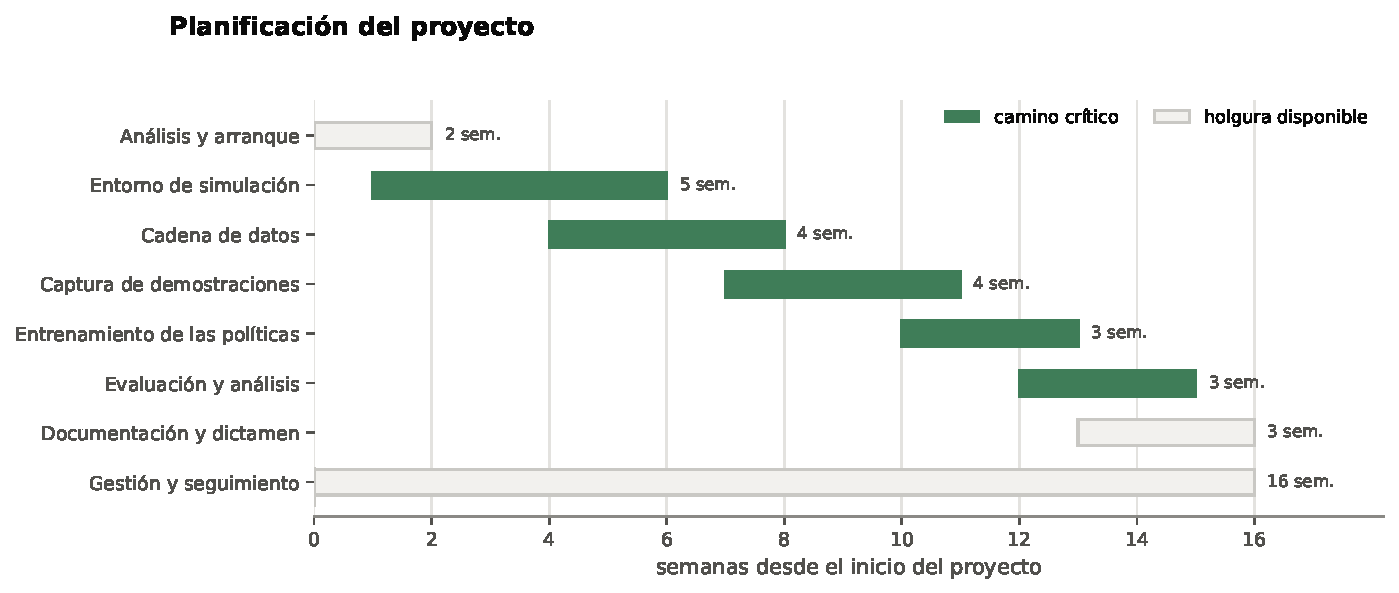
\includegraphics[width=\textwidth]{figuras/sistema/gantt.pdf}
  \caption[Planificación temporal del proyecto]{Planificación temporal del proyecto simulado, con
  indicación del camino crítico}
  \label{fig:gantt}
\end{figure}

El camino crítico —en verde en la figura \ref{fig:gantt}— es la secuencia T1 → T2 → T3 → T4 → T5. No
tiene holgura: un retraso de una semana en el entorno es una semana de retraso en el dictamen. Las
únicas tareas con holgura son las que no están en él: el análisis inicial, que puede comprimirse,
y la documentación, que puede absorber un retraso avanzando en paralelo con la evaluación. La
consecuencia para la gestión es que el esfuerzo de control se concentra en las dos primeras tareas
del camino, donde está la incertidumbre, y no en las últimas, donde el trabajo es predecible.


\section{Gestión de recursos}

\subsection{Especificación de recursos}

\textbf{Recursos humanos.} Cinco perfiles, ninguno a tiempo completo durante todo el proyecto: un
ingeniero de robótica sénior (T0, T1, T6), un técnico de teleoperación (T3), un ingeniero de
aprendizaje automático (T2, T4, y apoyo en T5), un ingeniero de pruebas (T5) y un jefe de proyecto
(T7). El técnico de teleoperación es el recurso más específico: debe ser una sola persona durante
toda la captura, porque el estilo del operador queda grabado en las demostraciones y dos estilos
dan un conjunto de datos peor que uno.

\textbf{Recursos materiales.} La estación de trabajo con sus dos aceleradoras y el visor de realidad
mixta, descritos en la tabla \ref{tab:presupuesto-hardware}, más una red local de baja latencia
entre ambos: la transmisión de vídeo estereoscópico al visor no tolera una red inalámbrica
saturada.

\textbf{Infraestructura.} Un contenedor con la pila de simulación, que aísla sus dependencias y
permite reconstruirlo; almacenamiento para el conjunto de datos y los puntos de control —del orden
de un terabyte—; y un repositorio de control de versiones con los cambios sobre el marco de
terceros conservados como parches.

\subsection{Asignación de recursos}

El cuello de botella es la \textbf{estación de trabajo}, que es única y la necesitan todas las
tareas del camino crítico. La asignación resuelve la contención por dos vías. La primera es la
separación por aceleradora: la GPU 0 queda dedicada a la teleoperación y la grabación durante las
sesiones de captura, porque la transmisión al visor no tolera compartir la GPU, y la GPU 1 corre en
paralelo la aplicación del fondo fotorrealista, los entrenamientos y las evaluaciones. La segunda es
la separación por horario: los trabajos largos y sin supervisión —reproducción de sesiones,
entrenamientos, bloques de cientos de tiradas— se lanzan por la noche, de modo que la máquina
produce veinticuatro horas y las personas la usan de día. Ambas prácticas salen del desarrollo real,
donde una noche de máquina cubrió los seis entrenamientos y las seiscientas tiradas de la curva de
eficiencia.

La carga humana está equilibrada por construcción: los perfiles se suceden a lo largo del camino
crítico —sénior, técnico, aprendizaje automático, pruebas, sénior— y solo el jefe de proyecto
acompaña todo el recorrido. El punto de solapamiento de personas está en las semanas 10 a 13,
cuando captura, entrenamiento y evaluación coinciden, y es donde la máquina, no las personas, marca
el ritmo.


\section{Gestión de riesgos}
\label{sec:riesgos}

\subsection{Identificación de riesgos}

El catálogo de riesgos de la tabla \ref{tab:riesgos} se ha construido a partir de los que
efectivamente se materializaron durante el desarrollo real, más los propios de cualquier proyecto
de esta naturaleza. Es una lista corta a propósito: ocho riesgos que se pueden vigilar valen más
que treinta que nadie revisa.

\begin{table*}[ht]
	\centering
	\caption{Catálogo de riesgos}
	\label{tab:riesgos}
	\makebox[\textwidth]{
		\begin{tabular}{|l|p{5.2cm}|p{7.6cm}|}
			\cline{1-3}
			Id & Riesgo & Causa y efecto \\ \hline
			R1 & Inestabilidad de la pila de realidad mixta & Fallos de configuración sin síntoma visible (transmisión en negro, sobreexposición, cierres al arrancar). Bloquea la captura \\
			R2 & Incompatibilidad entre versiones de bibliotecas & Las bibliotecas de aprendizaje fijan versiones incompatibles con el simulador. Rompe la evaluación o el entrenamiento \\
			R3 & Invalidación de datos ya capturados & Un cambio de decisión o un fallo silencioso del \textit{pipeline} obliga a descartar o regrabar sesiones \\
			R4 & Indisponibilidad de la estación de trabajo & Es única y compartida; una avería o un uso concurrente detiene el camino crítico \\
			R5 & Ampliación no controlada del alcance & Mejoras deseables —fondo fotorrealista, más tareas— desplazan el trabajo comprometido \\
			R6 & Pérdida de cambios sobre el marco de terceros & Modificaciones no versionadas sobre el simulador se destruyen al actualizarlo \\
			R7 & Baja del operador de teleoperación & Es una sola persona; su ausencia detiene la captura y cambiar de operador cambia los datos \\
			R8 & Resultados no concluyentes & La diferencia entre métodos es pequeña y el contraste no la acredita. Debilita el dictamen \\ \hline
		\end{tabular}
	}
\end{table*}

\subsection{Análisis de riesgos}

Cada riesgo se valora en probabilidad e impacto en una escala de uno a cinco, y su exposición es el
producto de ambos. La figura \ref{fig:riesgos} los sitúa en la matriz; la tabla
\ref{tab:analisis-riesgos} recoge la valoración, el plan de mitigación —lo que se hace para que no
ocurra— y el de contingencia —lo que se hace cuando ocurre.

\begin{figure}[htb]
\centering
  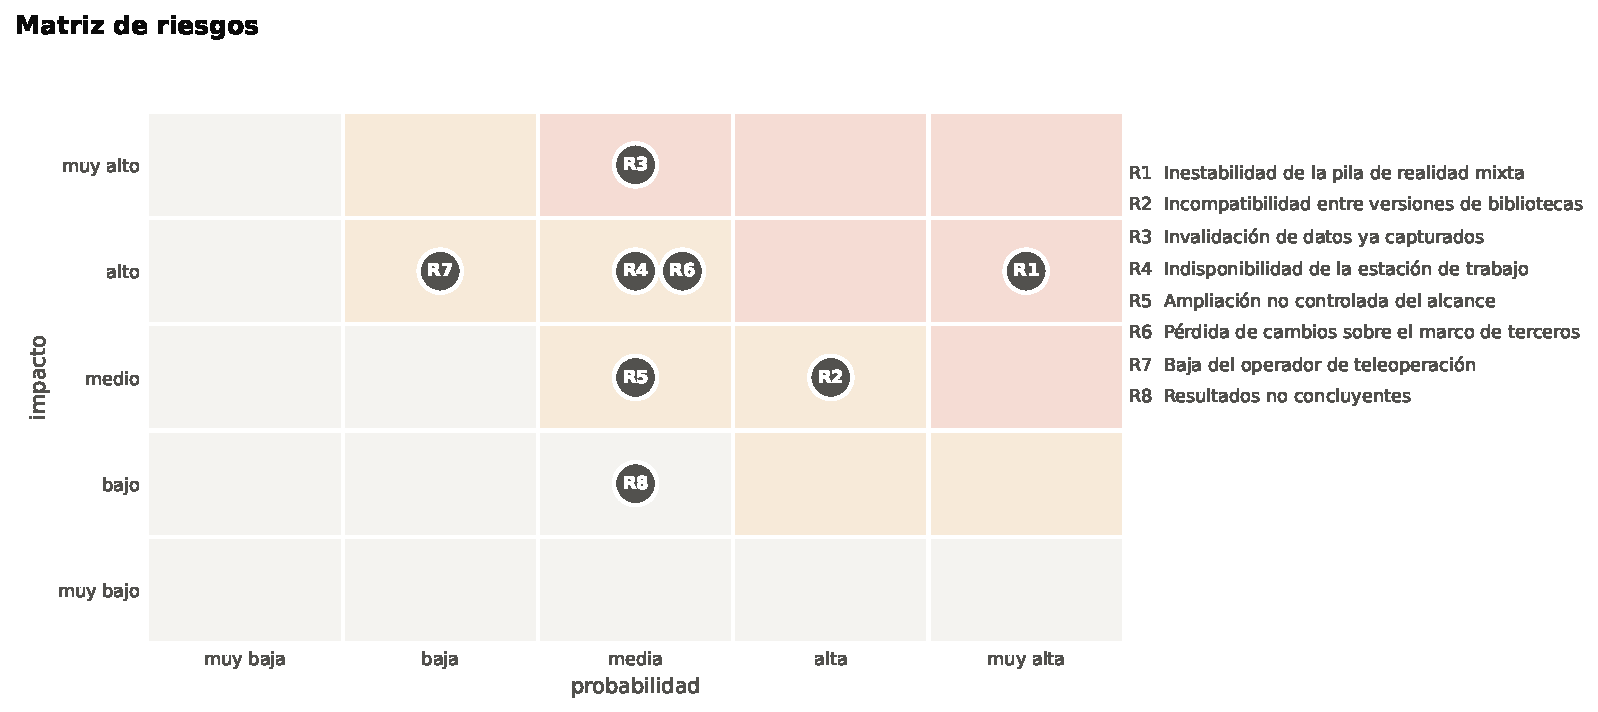
\includegraphics[width=\textwidth]{figuras/sistema/riesgos.pdf}
  \caption[Matriz de riesgos]{Matriz de riesgos del proyecto: probabilidad frente a impacto}
  \label{fig:riesgos}
\end{figure}

\begin{table*}[ht]
	\centering
	\caption{Análisis de riesgos: valoración, mitigación y contingencia}
	\label{tab:analisis-riesgos}
	\makebox[\textwidth]{
		\begin{tabular}{|l|c|c|c|p{5.4cm}|p{5.2cm}|}
			\cline{1-6}
			Id & P & I & P$\times$I & Mitigación & Contingencia \\ \hline
			R1 & 5 & 4 & 20 & Recetas de lanzamiento verificadas y documentadas; tabla de fallos conocidos; monitor en tercera persona para aislar fallos & Semanas de margen en T1; contingencia presupuestaria \\
			R2 & 4 & 3 & 12 & Un entorno de ejecución por método, aislado del simulador; versiones fijadas por escrito & Fijar la última versión compatible y no actualizar \\
			R3 & 3 & 5 & 15 & Verificar una demostración de extremo a extremo antes de grabar en bloque; decisiones de captura cerradas antes del conjunto definitivo & Tratar la sesión perdida como prueba del \textit{pipeline}; regrabar en sesiones de veinticinco \\
			R4 & 3 & 4 & 12 & Reparto por GPU y por horario; trabajos largos desatendidos y reanudables & Reordenar el plan hacia tareas sin máquina (documentación) \\
			R5 & 3 & 3 & 9 & Alcance escrito con exclusiones explícitas; toda ampliación pasa por el jefe de proyecto & Diferir la ampliación a un anexo o a una fase posterior \\
			R6 & 3 & 4 & 12 & Copia versionada de cada cambio como parche; sincronización periódica & Regenerar desde los parches \\
			R7 & 2 & 4 & 8 & Sesiones cortas y frecuentes; documentar el gesto de captura & Reprogramar T3; si se cambia de operador, regrabar el conjunto entero \\
			R8 & 3 & 2 & 6 & Diseño emparejado y tamaño muestral suficiente desde el inicio & Presentar el resultado con su incertidumbre; el dictamen es válido aunque no sea concluyente \\ \hline
		\end{tabular}
	}
\end{table*}

Los dos riesgos que dominan la matriz son R1 y R3, y son también los dos que se materializaron con
más coste en el desarrollo real: la pila de realidad mixta consumió sesiones enteras, y una sesión
de datos completa quedó invalidada por un fallo silencioso del proceso de reproducción antes de
que nadie lo advirtiera. La lección que incorpora el plan es la misma en ambos casos: verificar cada
etapa de extremo a extremo con datos reales antes de invertir esfuerzo en la siguiente, aunque
ello retrase el arranque de la captura. Es más barato perder una semana en T1 que una sesión en T3.


\chapter{Solución}
\label{Solución}

Este capítulo describe el sistema construido: qué se ha desarrollado, con qué arquitectura, cómo se
ha implementado y qué pruebas garantizan que cada eslabón hace lo que dice hacer. Es el capítulo más
extenso de la memoria porque el trabajo no consiste en aplicar un modelo a un conjunto de datos ya
existente, sino en construir la tarea, el conjunto de datos y el banco de evaluación desde cero.


\section{Descripción de la solución}

Visión de conjunto antes del detalle. Lo desarrollado es un \textbf{banco de comparación de
políticas de manipulación}: un entorno de simulación con una tarea instrumentada, una cadena de
captura y conversión de demostraciones, dos vías de entrenamiento que consumen el mismo conjunto de
datos, y un protocolo de evaluación que sirve a ambas a través de la misma interfaz.

\begin{figure}[htb]
\centering
  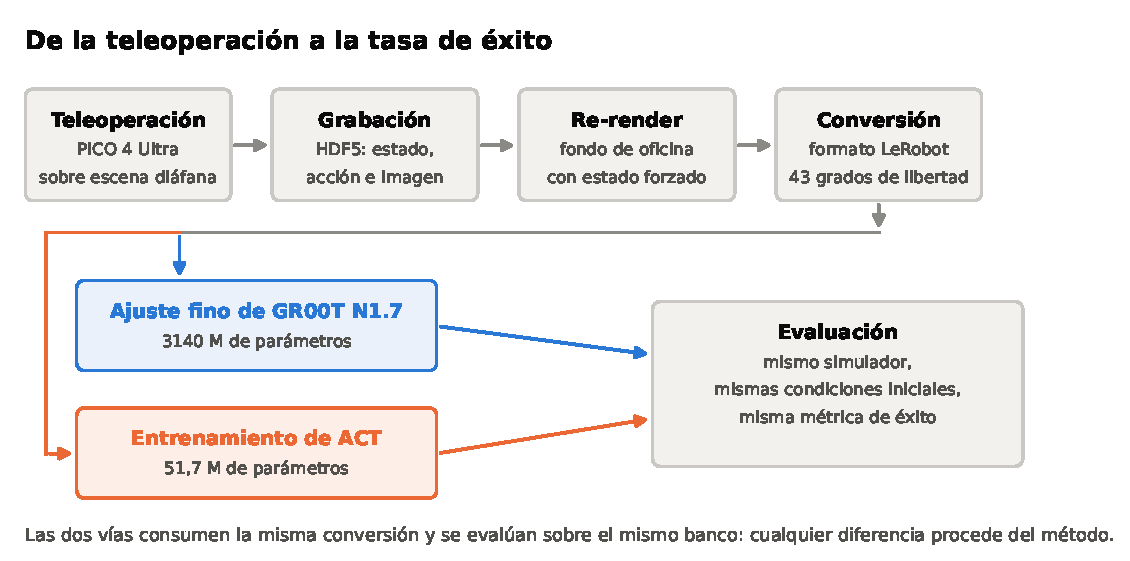
\includegraphics[width=\textwidth]{figuras/sistema/pipeline.pdf}
  \caption[Cadena completa del sistema]{Cadena completa: teleoperación, grabación, conversión,
  entrenamiento por las dos vías y evaluación sobre el mismo simulador}
  \label{fig:pipeline}
\end{figure}


\section{El proceso de desarrollo}

El desarrollo ha seguido un modelo iterativo e incremental, con ciclos cortos cerrados por una
verificación ejecutable. La justificación es específica del dominio: en una cadena de cinco etapas
donde cada una consume la salida de la anterior, un error silencioso en un eslabón temprano invalida
todo el trabajo posterior sin producir ningún síntoma visible. El desarrollo se ordena, por tanto,
de modo que cada etapa quede verificada antes de invertir esfuerzo en la siguiente.

\subsection{Análisis}

\subsubsection{Definición de requisitos}

Enumeración de los requisitos del sistema, divididos en funcionales y no funcionales.

\begin{table*}[ht]
	\centering
	\caption{Requisitos funcionales}
	\label{tab:requisitos-funcionales}
	\makebox[\textwidth]{
		\begin{tabular}{|l|p{11cm}|}
			\cline{1-2}
			Código & Descripción \\ \hline
			RF-01 & [PENDIENTE: la tarea debe poder teleoperarse y grabarse] \\
			RF-02 & [PENDIENTE: criterio de éxito objetivo y automático] \\
			RF-03 & [PENDIENTE: una sola conversión alimenta a los dos métodos] \\
			RF-04 & [PENDIENTE: banco de evaluación común e intercambiable] \\ \hline
		\end{tabular}
	}
\end{table*}

\begin{table*}[ht]
	\centering
	\caption{Requisitos no funcionales}
	\label{tab:requisitos-no-funcionales}
	\makebox[\textwidth]{
		\begin{tabular}{|l|p{11cm}|}
			\cline{1-2}
			Código & Descripción \\ \hline
			RNF-01 & [PENDIENTE: reproducibilidad] \\
			RNF-02 & [PENDIENTE: latencia compatible con el lazo de control] \\
			RNF-03 & [PENDIENTE: trazabilidad de datos y modelos] \\ \hline
		\end{tabular}
	}
\end{table*}

\subsubsection{Especificación de requisitos}

Análisis de los requisitos desde el punto de vista del comportamiento, la estructura y la
funcionalidad del sistema, con los casos de uso principales: capturar una sesión de demostraciones,
convertir un conjunto de datos, entrenar una política y evaluarla.

\subsection{Diseño}

\subsubsection{Diseño de sistema}

Arquitectura y tecnologías. El sistema se reparte entre un contenedor que aloja el simulador y dos
entornos de ejecución independientes para cada método de aprendizaje, comunicados con el simulador
mediante un protocolo de mensajería. Esa separación no es estética: las bibliotecas de aprendizaje
fijan versiones de sus dependencias que son incompatibles con las que exige el simulador, de modo
que instalarlas juntas rompería la herramienta necesaria para evaluar.

\begin{figure}[htb]
\centering
  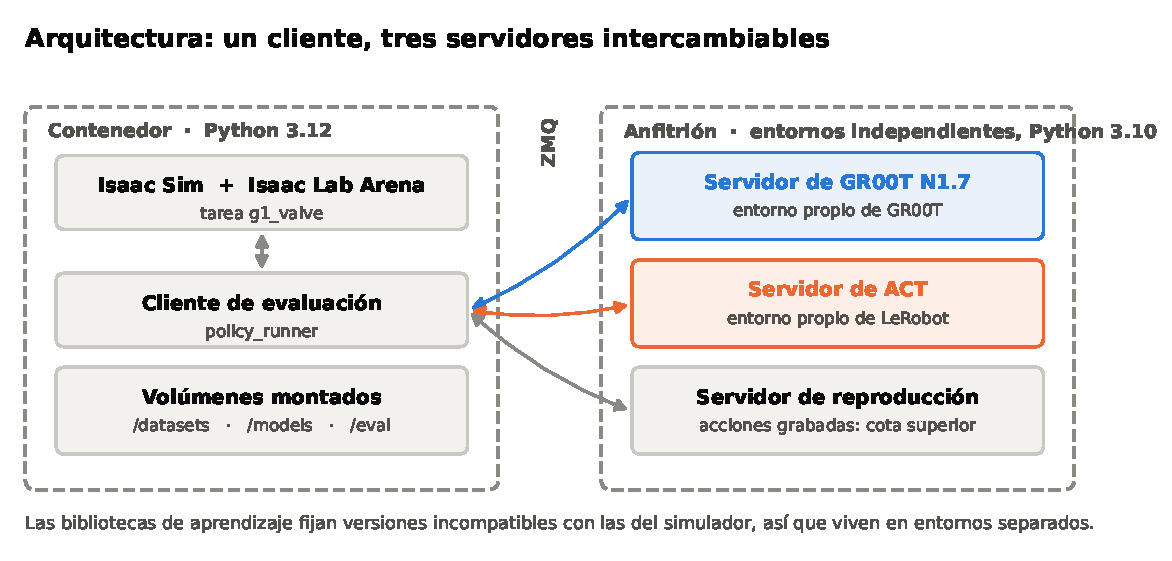
\includegraphics[width=\textwidth]{figuras/sistema/arquitectura.pdf}
  \caption[Arquitectura del sistema]{Arquitectura del sistema: contenedor de simulación, entornos de
  ejecución de cada política y comunicación entre ambos}
  \label{fig:arquitectura}
\end{figure}

\begin{table*}[ht]
	\centering
	\caption{Tecnologías empleadas y versiones}
	\label{tab:tecnologias}
	\makebox[\textwidth]{
		\begin{tabular}{|l|l|p{7cm}|}
			\cline{1-3}
			Componente & Versión & Función \\ \hline
			[PENDIENTE] & & \\ \hline
		\end{tabular}
	}
\end{table*}

\subsubsection{Diseño detallado}

Diseño de la tarea de simulación, de la representación de los datos y de la interfaz de las
políticas.

\paragraph{La tarea de simulación.} Escena, robot, válvula y criterio de éxito. Se detalla aquí la
elección de las dos disposiciones de la válvula, la aleatorización de su posición y el
procedimiento de medida con el que se han fijado todas las poses del entorno.

\begin{figure}[htb]
\centering
  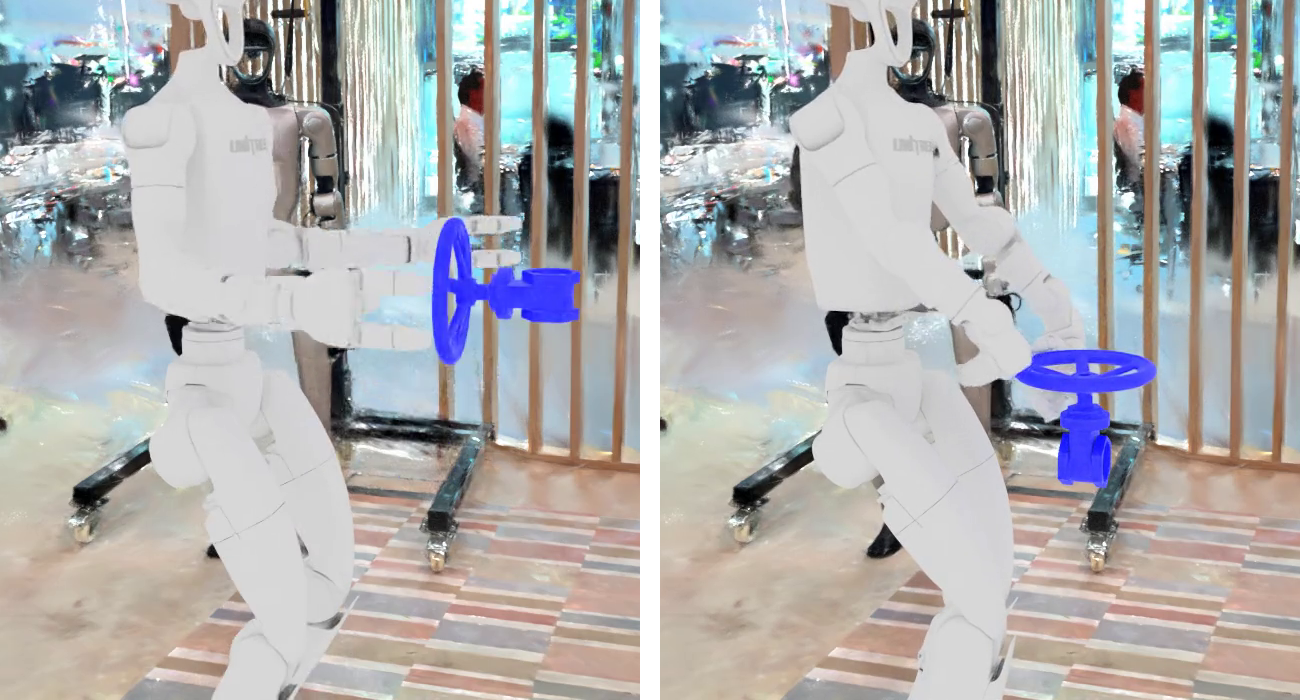
\includegraphics[width=\textwidth]{figuras/simulacion/disposiciones.png}
  \caption[Las dos disposiciones de la válvula]{Las dos disposiciones de la válvula: frontal, con el
  eje de giro horizontal, y cenital, con el eje vertical}
  \label{fig:disposiciones}
\end{figure}

\paragraph{El espacio de acción.} Composición de las veintitrés dimensiones que gobiernan al robot y
discusión de las que resultan degeneradas en el conjunto de datos.

\begin{figure}[htb]
\centering
  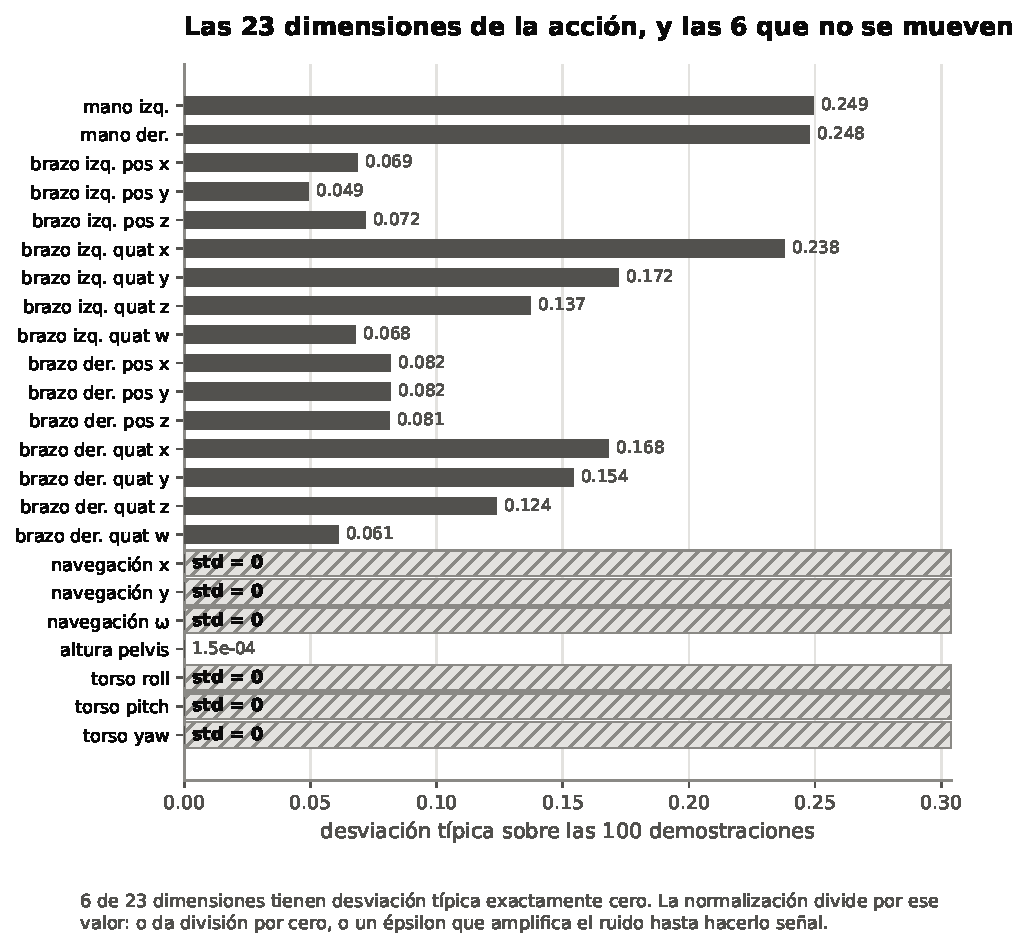
\includegraphics[width=\textwidth]{figuras/resultados/fig7_std_espacio_accion.pdf}
  \caption[Variabilidad de las dimensiones del espacio de acción]{Desviación típica de cada una de
  las veintitrés dimensiones del espacio de acción sobre el conjunto de datos definitivo}
  \label{fig:std-accion}
\end{figure}

\paragraph{El conjunto de datos.} Estructura del formato de almacenamiento y correspondencia entre
la acción de veintitrés dimensiones del simulador y el espacio articular de cuarenta y tres grados
de libertad que consumen las políticas. Se caracteriza aquí el conjunto capturado: cuántas
demostraciones tiene cada sesión, cómo se repartieron entre las dos disposiciones y cuánto dura
cada episodio.

\begin{figure}[htb]
\centering
  
\includegraphics[width=\textwidth]{figuras/resultados/fig5_reparto_disposiciones.pdf}
  \caption[Reparto de disposiciones por sesión]{Reparto de las dos disposiciones de la válvula en
  cada sesión de captura y en el conjunto acumulado}
  \label{fig:reparto-disposiciones}
\end{figure}

\begin{figure}[htb]
\centering
  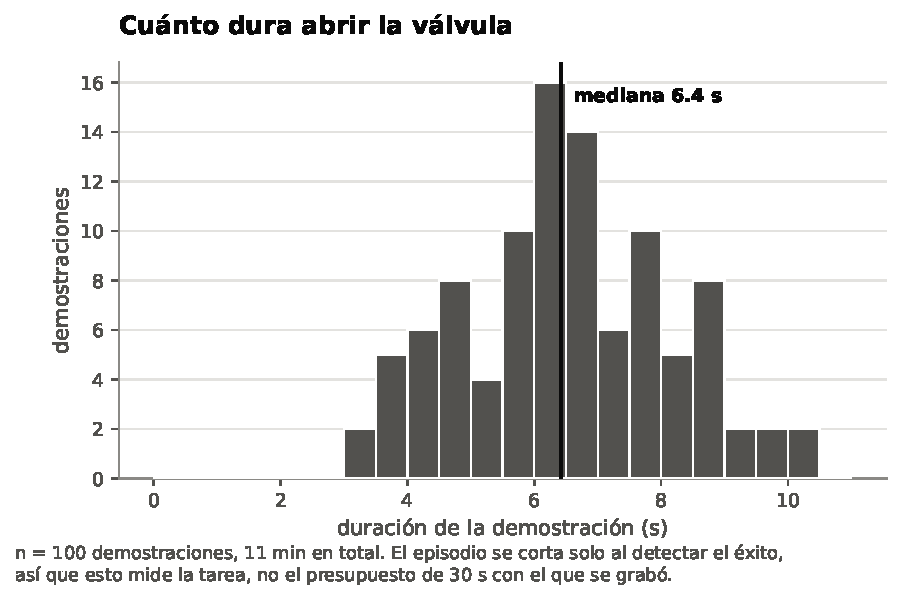
\includegraphics[width=\textwidth]{figuras/resultados/fig6_duracion_episodios.pdf}
  \caption[Duración de las demostraciones]{Distribución de la duración de las demostraciones
  capturadas}
  \label{fig:duracion-episodios}
\end{figure}

\subsection{Implementación}

Herramientas empleadas, organización del proyecto y peculiaridades de la implementación. Esta
sección recoge las decisiones técnicas que condicionaron el resultado y los problemas que hubo que
resolver para que la cadena funcionase: el reescalado de los límites de la articulación de la
válvula, la altura de aparición del robot, la sincronización del sensor de imagen con la
construcción del entorno, la elección del dispositivo de física durante la captura y el
procedimiento de reaplicación del fondo fotorrealista sobre demostraciones ya grabadas.

\begin{figure}[htb]
\centering
  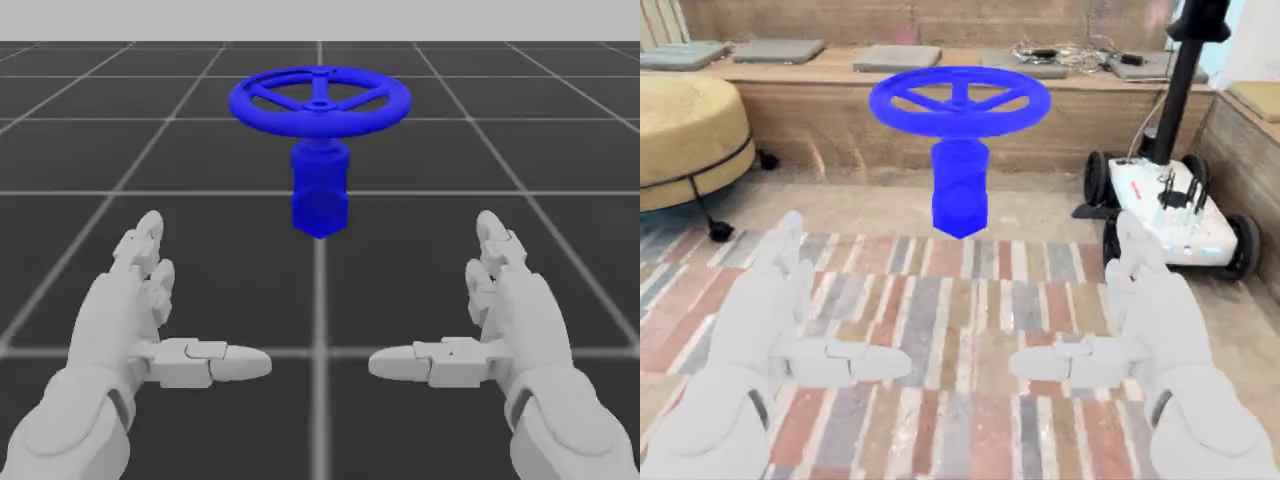
\includegraphics[width=\textwidth]{figuras/simulacion/escenas.png}
  \caption[Escena de captura y escena del conjunto de datos]{Escena diáfana empleada durante la
  teleoperación, frente a la misma demostración con el fondo de oficina reconstruido, que es la que
  llega al conjunto de datos}
  \label{fig:escenas}
\end{figure}

\subsection{Pruebas}

Pruebas realizadas sobre cada eslabón de la cadena, con el resultado de cada una. La pieza central
es la reproducción de las acciones grabadas como cota superior del sistema: si reproducir las
órdenes de una demostración no abre la válvula, ninguna política entrenada sobre ellas lo hará, y
eso debe saberse antes de invertir en la captura masiva.

\begin{table*}[ht]
	\centering
	\caption{Pruebas de verificación de la cadena}
	\label{tab:pruebas}
	\makebox[\textwidth]{
		\begin{tabular}{|l|p{8cm}|l|}
			\cline{1-3}
			Prueba & Qué verifica & Resultado \\ \hline
			[PENDIENTE] & & \\ \hline
		\end{tabular}
	}
\end{table*}


\section{El producto del desarrollo}

Descripción del entregable: el repositorio, su organización, la documentación de lanzamiento y de
entrenamiento, y la forma de ejecutar cada etapa. Se incluyen ejemplos de la interfaz de captura tal
como la ve el operador y de la vista que recibe la política.

\begin{figure}[htb]
\centering
  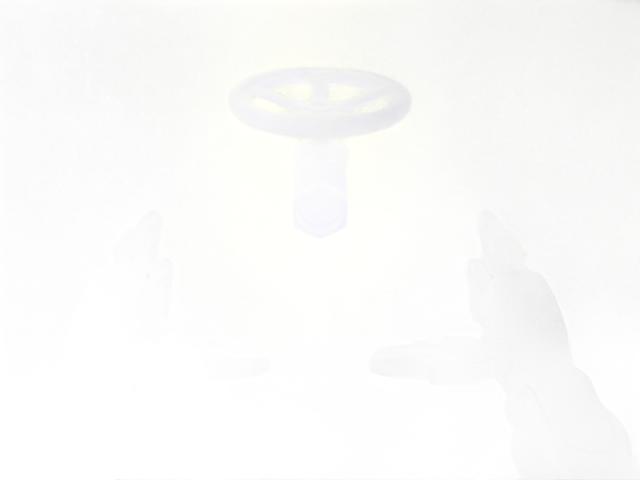
\includegraphics[width=.7\textwidth]{figuras/simulacion/camara_robot.png}
  \caption[Vista de la cámara del robot]{Vista de la cámara de cabeza del robot, que es la única
  entrada visual que recibe la política}
  \label{fig:camara-robot}
\end{figure}


\chapter{Evaluación}
\label{Evaluación}

Este capítulo demuestra la validez de la solución construida. Describe primero el protocolo
experimental —qué se mide, cómo se mide y por qué el diseño permite atribuir las diferencias
observadas al método y no al montaje— y analiza después los resultados de los tres experimentos
realizados: la comparación principal entre las dos políticas, la curva de eficiencia en datos y la
medida de latencia de inferencia.

Se ha puesto especial cuidado en separar lo que los datos sostienen de lo que sugieren. Varias de
las conclusiones de este capítulo son deliberadamente más débiles de lo que las cifras brutas
invitarían a escribir, y en cada caso se explica por qué.


\section{Proceso de evaluación}

\subsection{Forma de evaluación}

\subsubsection{Métricas}

Se emplean dos métricas, ambas registradas automáticamente por el simulador:

\begin{description}
	\item[tasa de éxito]: proporción de episodios en los que la válvula supera media vuelta de
	apertura. Es la métrica principal.
	\item[tasa de movimiento de la articulación]: proporción de episodios en los que la válvula
	llega a moverse, con independencia de cuánto. Distingue el fallo por no completar el giro del
	fallo por no encontrar siquiera la válvula.
\end{description}

Se acompañan del ángulo final alcanzado por el volante, que permite ver la distribución de los
fallos en lugar de reducirlos a un contador.

\subsubsection{El banco es común a las dos políticas}

Las dos políticas se sirven como procesos independientes que implementan la misma interfaz de
comunicación con el simulador. El comando que lanza la evaluación es idéntico para ambas hasta el
último carácter: mismo entorno, mismo \textit{embodiment}, misma semilla y mismo presupuesto de
episodio. Lo único que cambia es qué proceso atiende la petición. Cualquier diferencia en la tasa de
éxito procede, por construcción, de la política.

\subsubsection{El diseño es emparejado}

Las condiciones iniciales de cada episodio —posición y orientación de la válvula— se generan a
partir de una semilla fija, de modo que la tirada $i$ de una política se enfrenta exactamente a la
misma escena que la tirada $i$ de la otra. Se ha verificado que las poses registradas coinciden
hasta el noveno decimal.

Esto convierte el experimento en un diseño de medidas emparejadas, y el contraste apropiado es la
\textbf{prueba exacta de McNemar} sobre los casos discordantes. Emplear una comparación de
proporciones independientes desaprovecharía la información del emparejamiento y sobreestimaría la
incertidumbre. Los intervalos de confianza de las tasas individuales se calculan por el método de
Wilson, que a diferencia del intervalo normal se mantiene dentro de $[0,1]$ con proporciones
próximas a los extremos, que es justo donde caen estos resultados.

\subsection{Casos de prueba}

\subsubsection{Ensayo previo de la cadena}

Pasada completa con veinticinco demostraciones de una sola disposición, con el único objetivo de
recorrer la cadena entera con datos reales y localizar dónde se rompe. Ambas políticas alcanzaron
diez éxitos de diez, lo que \textbf{no distingue nada}: sirve para afirmar que la cadena funciona,
no para comparar métodos.

\subsubsection{Comparación principal}

Doscientas tiradas por política, en dos bloques de cien con semillas distintas, sobre las políticas
entrenadas con las cien demostraciones definitivas.

\subsubsection{Curva de eficiencia en datos}

Reentrenamiento de ambos métodos sobre subconjuntos \textbf{estratificados y anidados} de
veinticinco y cincuenta demostraciones, y evaluación de las seis configuraciones resultantes sobre
las mismas cien condiciones iniciales. La estratificación es esencial: las primeras sesiones
grabadas se escoraron hacia la disposición difícil, de modo que tomar «las primeras veinticinco»
habría confundido \textit{menos datos} con \textit{más disposición difícil} y la curva habría caído
por el motivo equivocado.

\subsubsection{Latencia de inferencia}

Medida del tiempo de cálculo de cada bloque de acciones en lazo cerrado dentro del simulador, con
las observaciones reales y no con entradas sintéticas, y contraste contra el presupuesto que impone
el lazo de control.


\section{Análisis de resultados}

\subsection{Convergencia del entrenamiento}

\begin{figure}[htb]
\centering
  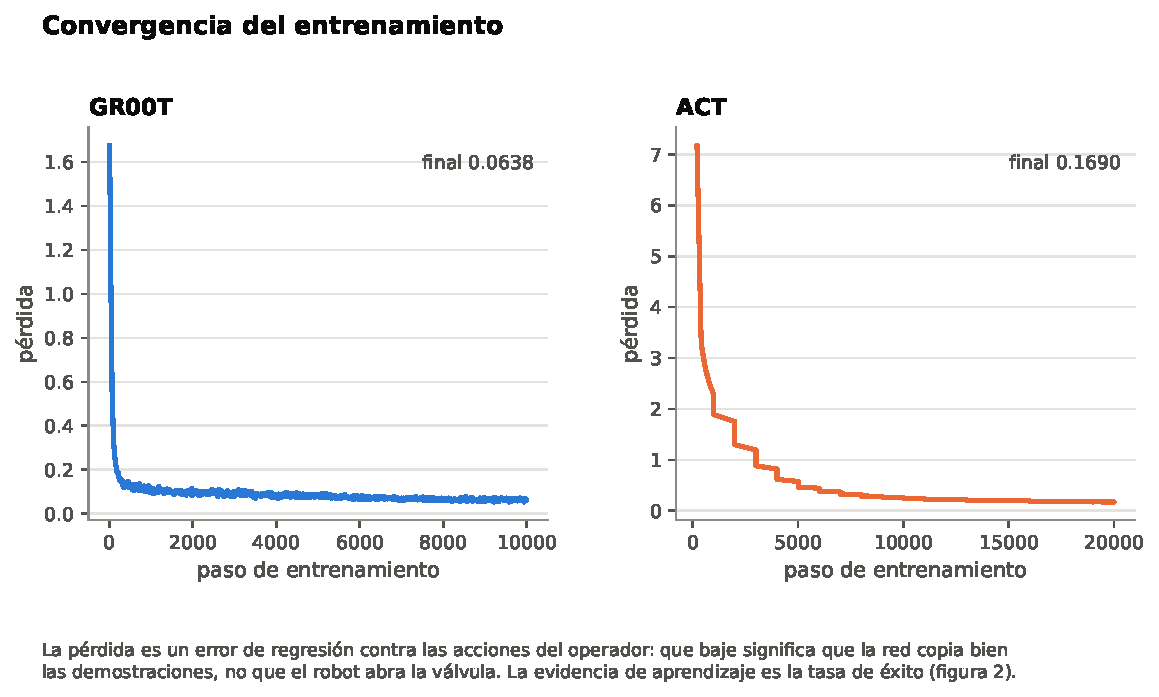
\includegraphics[width=\textwidth]{figuras/resultados/fig1_curvas_perdida.pdf}
  \caption[Convergencia del entrenamiento]{Convergencia del entrenamiento de ambos métodos, en
  paneles separados}
  \label{fig:perdida}
\end{figure}

Ambos entrenamientos convergen. Conviene subrayar, no obstante, que la pérdida en aprendizaje por
imitación es un error de regresión contra las acciones del operador: que baje significa que la red
copia bien las demostraciones, no que el robot abra la válvula. Una política puede exhibir una
pérdida excelente y una tasa de éxito nula si aprende la media de las demostraciones. La evidencia
de aprendizaje es la tasa de éxito en simulación; las curvas solo acreditan que la optimización
convergió. Las dos pérdidas, además, no son comparables entre sí, y por eso van en paneles
separados.

\subsection{Comparación principal}

\begin{table*}[ht]
	\centering
	\caption{Resultado sobre doscientas tiradas por política}
	\label{tab:resultado-principal}
	\makebox[\textwidth]{
		\begin{tabular}{|l|c|c|c|c|c|}
			\cline{1-6}
			Política & Tiradas & Éxito & IC 95\,\% & Movió la válvula & Ángulo medio \\ \hline
			GR00T N1.7 & 200 & \textbf{92\,\%} (185/200) & 88--95\,\% & 100\,\% & 177\textdegree \\
			ACT & 200 & \textbf{86\,\%} (172/200) & 81--90\,\% & 100\,\% & 173\textdegree \\ \hline
		\end{tabular}
	}
\end{table*}

\begin{figure}[htb]
\centering
  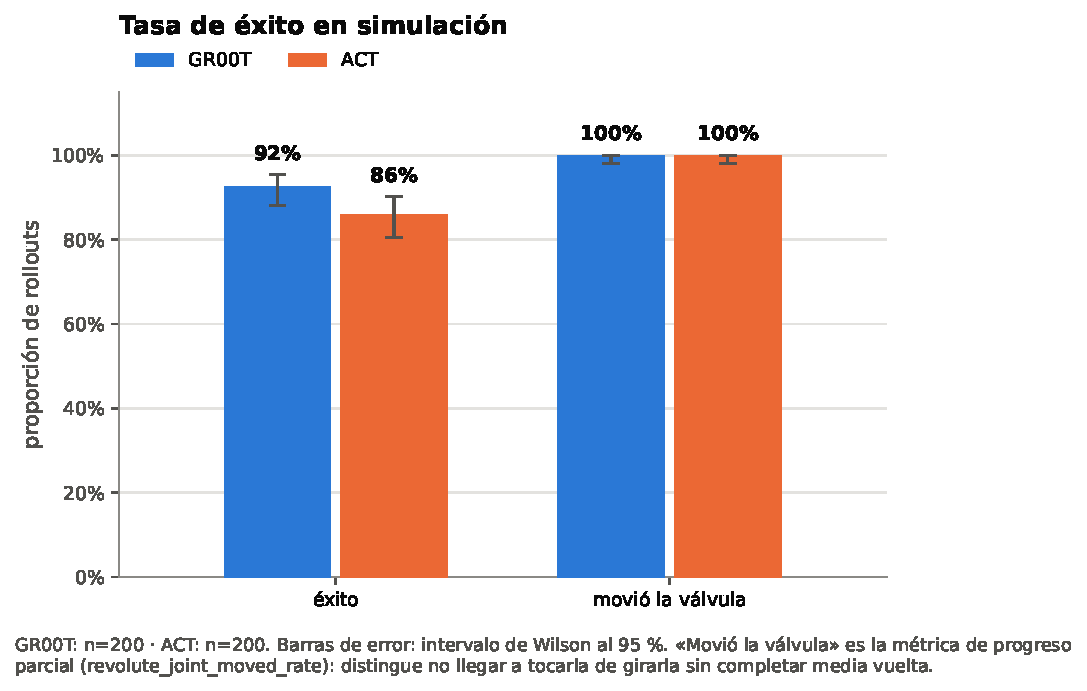
\includegraphics[width=\textwidth]{figuras/resultados/fig2_tasa_exito.pdf}
  \caption[Tasa de éxito de ambas políticas]{Tasa de éxito de ambas políticas con intervalos de
  confianza de Wilson al 95\,\%}
  \label{fig:tasa-exito}
\end{figure}

\subsubsection{El contraste emparejado}

De las doscientas tiradas, ciento sesenta las resuelven ambas políticas, veinticinco solo GR00T,
doce solo ACT y tres ninguna. La prueba exacta de McNemar sobre los treinta y siete casos
discordantes arroja $p = 0{,}047$.

\textbf{Ese valor cruza el umbral del 5\,\% por un solo episodio y es frágil.} Un reparto de
veinticuatro contra trece daría $p = 0{,}099$, y de veinticinco contra trece, $p = 0{,}073$. La
afirmación que los datos sostienen es que \textit{GR00T va consistentemente por delante en los dos
bloques y la diferencia se aproxima a la significación estadística}; afirmar que GR00T es
significativamente mejor que ACT sería sobreinterpretar el resultado.

\subsubsection{Dónde vive la diferencia}

\begin{figure}[htb]
\centering
  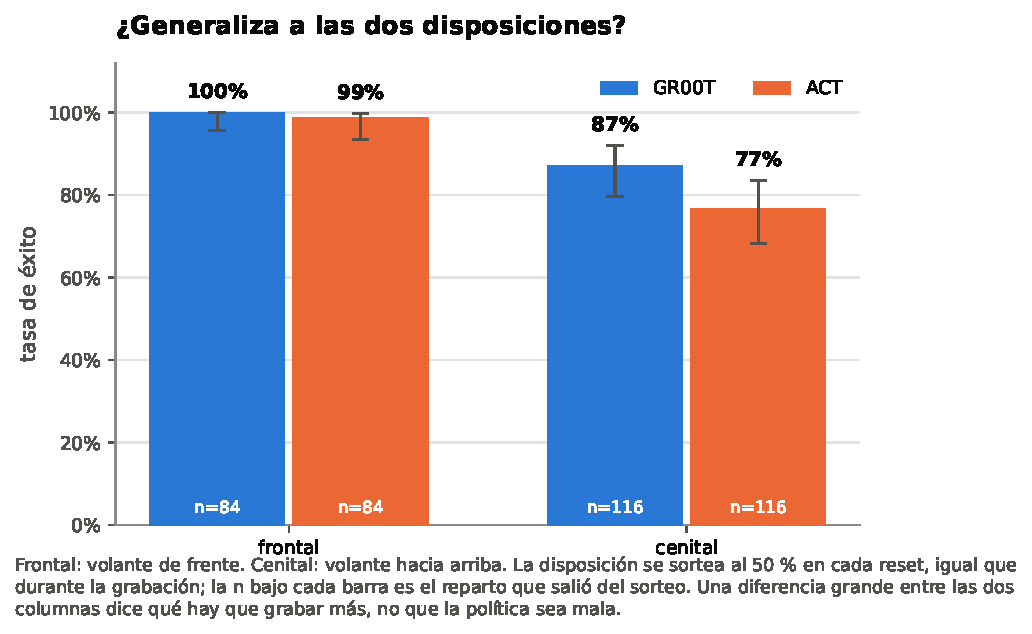
\includegraphics[width=\textwidth]{figuras/resultados/fig4_exito_por_disposicion.pdf}
  \caption[Tasa de éxito por disposición de la válvula]{Tasa de éxito de cada política separada por
  disposición de la válvula}
  \label{fig:por-disposicion}
\end{figure}

Lo que sí resulta significativo, y con mucho margen, es el efecto de la disposición: ambas políticas
son claramente peores con la válvula en posición cenital. Y toda la diferencia entre métodos vive
ahí: treinta y seis de los treinta y siete casos discordantes son cenitales, mientras que la
disposición frontal está saturada para las dos. La afirmación defendible es, por tanto, que
\textit{GR00T aguanta algo mejor la disposición difícil}, no que sea mejor en general.

\subsection{Distribución de los fallos}

\begin{figure}[htb]
\centering
  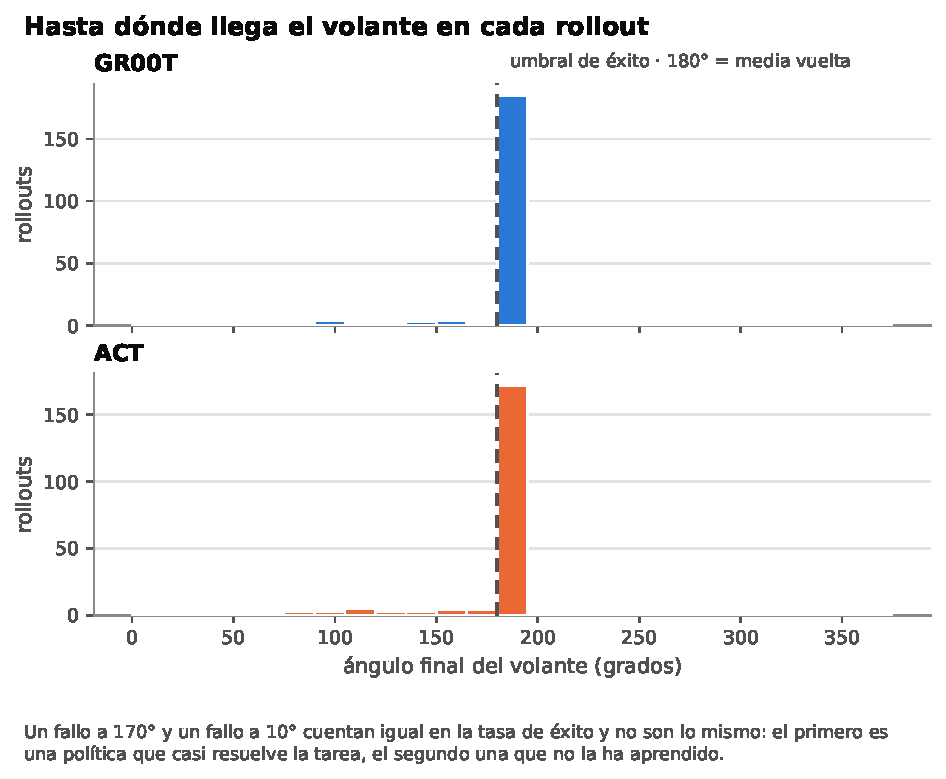
\includegraphics[width=\textwidth]{figuras/resultados/fig3_distribucion_angulo.pdf}
  \caption[Distribución del ángulo final alcanzado]{Distribución del ángulo final alcanzado por el
  volante, con el umbral de éxito marcado}
  \label{fig:angulos}
\end{figure}

La tasa de movimiento de la articulación resulta del 100\,\% para ambas políticas en las
cuatrocientas tiradas, de modo que no discrimina en esta comparación. Pero es en sí misma un
resultado: no hay ni un solo episodio en el que el robot no llegue a alcanzar la válvula. Todos los
fallos son de \textit{no completar media vuelta}, nunca de \textit{no encontrarla}.

\subsection{Eficiencia en datos}

\begin{figure}[htb]
\centering
  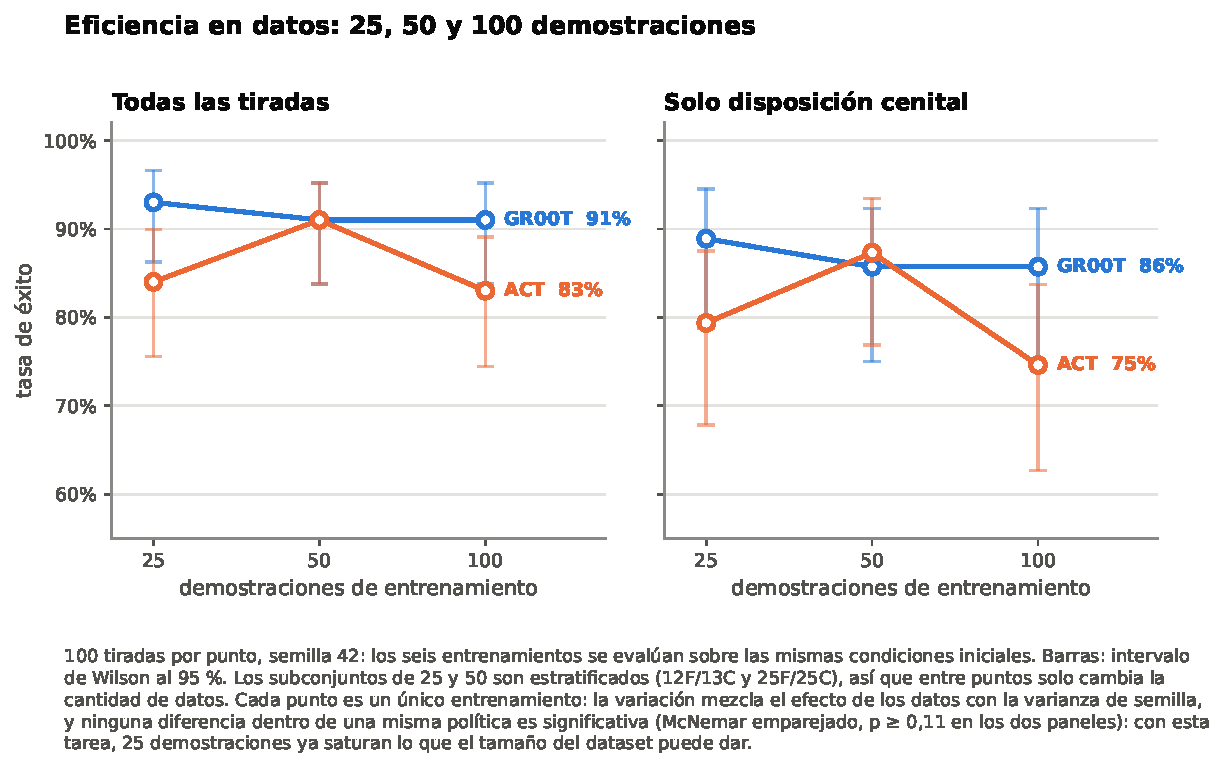
\includegraphics[width=\textwidth]{figuras/resultados/fig8_curva_eficiencia.pdf}
  \caption[Curva de eficiencia en datos]{Tasa de éxito frente al número de demostraciones de
  entrenamiento, en el total de las tiradas y restringida a la disposición cenital}
  \label{fig:eficiencia}
\end{figure}

La hipótesis que justifica el empleo de un modelo fundacional era que GR00T se despegara con pocas
demostraciones y ACT necesitara más. \textbf{No se observa.} Ninguna diferencia dentro de una misma
política resulta significativa. El resultado es negativo y es el más útil del experimento: el
margen de fallo restante \textbf{no es un problema de cantidad de datos}, sino de su composición.

Debe leerse con una cautela que se hace explícita: cada punto de la curva corresponde a un único
entrenamiento, de modo que la variación entre puntos mezcla el efecto de los datos con la varianza
de semilla del propio entrenamiento.

\subsection{Latencia de inferencia}

\begin{figure}[htb]
\centering
  
\includegraphics[width=\textwidth]{figuras/resultados/fig9_latencia.pdf}
  \caption[Coste de inferencia frente al presupuesto de tiempo real]{Coste de inferencia de cada
  política frente al presupuesto que impone el lazo de control}
  \label{fig:latencia}
\end{figure}

La diferencia de sesenta y un veces en número de parámetros se traduce en diez veces en latencia, y
aun así ambas políticas caben holgadamente dentro del presupuesto. La latencia no es, en esta tarea
y sobre este equipamiento, un argumento en contra del modelo fundacional.

\subsection{Amenazas a la validez}

Discusión honesta de los límites del experimento: una sola tarea, una sola semilla de entrenamiento
por configuración, ausencia de validación sobre robot físico, y el hecho de que las demostraciones
terminan justo al cruzar el umbral de éxito, lo que hace que parte de los fallos sean casi-éxitos
por construcción del protocolo de captura.


\mychapter{1}{Conclusión}
\markboth{CONCLUSIÓN}{}

Recapitulación de lo obtenido y valoración personal del trabajo. La conclusión de fondo se puede
enunciar en una frase: sobre esta tarea, el modelo fundacional va por delante de la política clásica
por un margen pequeño y difícil de acreditar estadísticamente, mientras que la variable que sí
domina el resultado —con dos contrastes por debajo de $p = 0{,}001$— es la disposición de la
válvula. Es un resultado menos vistoso que «el modelo grande gana», y bastante más útil para quien
tenga que decidir dónde invertir el esfuerzo.


\subsection*{Aportaciones realizadas}

Enumeración de lo aportado por el trabajo:

\begin{itemize}
	\item Una tarea de manipulación industrial instrumentada y reproducible sobre el humanoide
	Unitree G1, con criterio de éxito objetivo, poses medidas y variabilidad controlada.
	\item Un conjunto de cien demostraciones teleoperadas, con dos disposiciones de la válvula y
	fondo fotorrealista aplicado por reproducción.
	\item Un banco de comparación que sirve a dos familias de políticas a través de la misma
	interfaz, lo que permite atribuir las diferencias al método.
	\item Una comparación emparejada con el contraste estadístico apropiado, y la caracterización
	del coste de cada método en datos y en latencia.
	\item El hallazgo, negativo pero accionable, de que la limitación dominante en esta tarea no es
	la cantidad de demostraciones sino su composición.
\end{itemize}

\subsection*{Trabajos futuros}

Líneas de continuación: reequilibrar el conjunto de datos hacia la disposición difícil, repetir los
entrenamientos con varias semillas para separar el efecto de los datos de la varianza del
entrenamiento, eliminar las dimensiones degeneradas del espacio de acción, ampliar a más de una
tarea y, sobre todo, validar sobre robot físico.

\subsection*{Problemas encontrados}

Relato de los obstáculos que condicionaron el desarrollo y de cómo se resolvieron. Son en buena
medida los que explican el reparto real del esfuerzo, muy escorado hacia la construcción de la
cadena frente al entrenamiento de los modelos.

\section*{Opiniones personales}

Valoración personal del trabajo: qué se ha aprendido, qué se haría de otra manera y qué percepción
deja el estado actual de los modelos fundacionales para robótica frente a las alternativas
específicas.



%%%% BIBLIOGRAFÍA %%%%
\renewcommand\bibname{Lista de referencias}

\bibliography{referencias}
\bibliographystyle{unsrt} %plain %apalike


%%%% ANEXOS %%%%
\renewcommand{\appendixname}{Anexo}
\appendix

\chapter{Control de versiones}
\label{Control de versiones}

Descripción del control de versiones del proyecto: el repositorio propio que se entrega, la rama de
trabajo sobre el marco de simulación de terceros y el mecanismo que mantiene sincronizadas ambas
copias.

\section{Organización del repositorio}

Estructura de directorios del entregable y criterio de qué se versiona y qué no. En particular, por
qué los conjuntos de datos y los puntos de control de los modelos quedan fuera del repositorio.

\section{Los cambios sobre el marco de simulación}

El trabajo modifica ficheros de un proyecto de terceros. Esos cambios se conservan como parches
generados contra la base de la versión oficial, y no como copias completas, para que quede
explícito qué se ha tocado y para poder rebasarlos sobre versiones posteriores.

\begin{table*}[ht]
	\centering
	\caption{Parches aplicados sobre el marco de simulación}
	\label{tab:parches}
	\makebox[\textwidth]{
		\begin{tabular}{|l|p{10cm}|}
			\cline{1-2}
			Parche & Qué cambia \\ \hline
			[PENDIENTE] & \\ \hline
		\end{tabular}
	}
\end{table*}

\section{Historial de desarrollo}

Resumen del historial de confirmaciones, con el criterio seguido para los mensajes y para el reparto
del trabajo en incrementos verificables.


\chapter{Seguimiento de proyecto fin de máster}
\label{Seguimiento de proyecto fin de máster}

Seguimiento del trabajo real, por oposición a la simulación de gestión empresarial que recoge el
capítulo \ref{Gestión de proyecto software}.

\section{Forma de seguimiento}

Mecanismo de seguimiento empleado: reuniones con el tutor, documentación continua del estado del
proyecto en el propio repositorio y registro de decisiones con su fecha y su justificación.

\section{Planificación inicial}

Planificación prevista al comienzo del trabajo, con sus hitos.

\section{Planificación final}

Planificación realmente ejecutada y análisis de las desviaciones. Se documentan aquí las dos
decisiones que más alteraron el plan: la reducción del conjunto de datos previsto una vez se
comprobó que el tamaño no era el factor limitante, y la incorporación del fondo fotorrealista, que
inicialmente estaba fuera de alcance.

\begin{table*}[ht]
	\centering
	\caption{Desviaciones entre la planificación inicial y la final}
	\label{tab:desviaciones}
	\makebox[\textwidth]{
		\begin{tabular}{|p{5cm}|p{5cm}|p{5cm}|}
			\cline{1-3}
			Previsto & Realizado & Causa de la desviación \\ \hline
			[PENDIENTE] & & \\ \hline
		\end{tabular}
	}
\end{table*}


\chapter{Protocolo de evaluación}
\label{Protocolo de evaluación}

La plantilla reserva este anexo a los cuestionarios empleados durante la fase de evaluación. En este
trabajo \textbf{no procede}: la evaluación no se basa en la valoración subjetiva de usuarios, sino en
la ejecución automatizada de casos de prueba dentro del simulador, con un criterio de éxito medido
por el propio entorno. En su lugar se documenta aquí el protocolo experimental completo, que cumple
la misma función de permitir que un tercero reproduzca la evaluación.

\section{Condiciones de la evaluación}

Parámetros fijos de toda evaluación: entorno, \textit{embodiment}, fondo, presupuesto de episodio,
semillas y número de tiradas. Se justifica cada uno.

\section{Procedimiento}

Secuencia de pasos de una tirada de evaluación, desde el arranque del proceso que sirve la política
hasta la escritura del fichero de resultados.

\section{Registro de resultados}

Estructura del fichero de resultados y campos que se extraen de él para el análisis.

\begin{table*}[ht]
	\centering
	\caption{Campos registrados por episodio}
	\label{tab:campos-registro}
	\makebox[\textwidth]{
		\begin{tabular}{|l|p{10cm}|}
			\cline{1-2}
			Campo & Contenido \\ \hline
			[PENDIENTE] & \\ \hline
		\end{tabular}
	}
\end{table*}

\section{Análisis estadístico}

Procedimiento de análisis: cálculo de las tasas y sus intervalos de Wilson, emparejamiento de las
tiradas entre políticas, prueba exacta de McNemar sobre los casos discordantes y contraste de Fisher
para el efecto de la disposición.



\end{document}
